%% bare_jrnl.tex
%%
%% ============================================================
%% DRAFT pass. Full prose for Abstract, Introduction, Prior Work, Background,
%% and Methodology (deep). Results/Discussion is scaffolded with framing prose and
%% [bracketed] placeholders -- no experimental numbers are invented.
%% Figures point to their drafted assets in figures/; captions describe intended content.
%% Conventions:
%%   - \todo{...} = open TODO needing data/decision (formerly \sh{...}; all SH: notes converted).
%%   - "% NOTE:" = assumption or verify-before-submission flag.
%% references.bib: carry entries from the ISRR + IROS submissions; cite keys below are
%% placeholders matching those bibliographies.
%% ============================================================

% \documentclass[conference]{IEEEtran} 
\documentclass[10pt, conference]{IEEEtran} 
% \def\IEEEtitletopspace{18pt} % This avoids errors when submitting

\makeatletter
\pdfminorversion=4
\usepackage[margin=0.75in]{geometry}
\usepackage{ifpdf}
\usepackage{cite}
\bibliographystyle{unsrt}
\usepackage{amsmath}
\usepackage{algorithm}
\usepackage{multirow}
\usepackage[noend]{algpseudocode}
\ifCLASSINFOpdf
   \usepackage[pdftex]{graphicx}
 \else
\fi
\usepackage{upgreek}
\usepackage{dblfloatfix}
\usepackage{xcolor}
\usepackage{hyperref}
\usepackage{amssymb}
\usepackage{soul}
\usepackage{hhline}
\usepackage{booktabs}
\usepackage{float}
\hypersetup{
    colorlinks=true,
    linkcolor=blue,
    filecolor=magenta,
    urlcolor=cyan,
    citecolor=cyan,
}
\IEEEoverridecommandlockouts

\setlength{\textfloatsep}{1\baselineskip plus 0.2\baselineskip minus 0.5\baselineskip}

\newcommand{\cdo}[1]{\textcolor{red}{CDO: #1}}
\newcommand{\jx}[1]{\textcolor{blue}{JX: #1}}
\newcommand{\sh}[1]{\textcolor{orange}{SH: #1}}
\newcommand{\todo}[1]{\textcolor{orange}{\textbf{TODO: #1}}}

\renewcommand\IEEEkeywordsname{Keywords}

% ALTERNATE TITLES (foreground the safety contribution rather than overlapping ISRR):
% Probing for Properties: 
%   - "Tip Without Toppling: A Criticality-Aware Safety Framework for Multi-Modal
%      Non-Prehensile Parameter Estimation"
%   - "Safe Press-and-Pull: Managing Toppling and Press-Induced Slippage for
%      Shape-Agnostic Estimation of Mass, Center of Mass, and Friction"

\title{\LARGE \bf Criticality-Aware Safety Framework for Shape-Agnostic Estimation of Physical Properties by Press-and-Pull Tipping}

\begin{document}

\author{ Steven M. Hyland, Jing Xiao, and Cagdas D. Onal \\ \thanks{The authors are affiliated with the Robotics Engineering Department, Worcester Polytechnic Institute, MA 01609, USA. Correspondence: \texttt{smhyland@wpi.edu}.} }

\maketitle

\begin{abstract}
% NOTE: results-agnostic. Fill [bracketed] numbers from the journal experiments.
Safe manipulation depends on a small set of physical parameters: mass, center of mass (CoM), and the object--surface friction coefficient, which together determine an object's behavior during interaction, and that cannot be read reliably from vision alone. These parameters are often provided to robot controlllers and may be recovered through robotic interaction, although most methods do not consider the object's and the environment's safety. Specifically, under tipping regimes, the very contact forces used to control tipping can cause unexpected sliding at the object--table contact, risking an uncontrolled fall. We present a criticality-aware safety framework for non-prehensile parameter estimation that identifies this single governing hazard and certifies an interaction against it. The press-and-pull tipping primitive pins a well-defined pivot by using the object's own support surface as a passive grasp. We formalize an admissible interaction set under a single no-slip constraint and derive a safety margin that bounds the distance to that hazard across the entire tipping arc. We show that our safety margin permits deliberately crossing the nominal toppling angle when feasible, thereby improving the accuracy of the estimated parameters; we also expose the resulting safety--accuracy tradeoff. The framework recovers mass, CoM height, and friction in closed form from limited interactions without a grasp, shape prior, or a learned model. We validate on an industrial arm with combined wrist-mounted force/torque sensing and world-fixed depth imaging over \todo{N} objects spanning designed primitives with exact ground truth and irregular everyday items. The validation set spans controlled parametric sweeps over CoM position, base fillet radius, and pivot geometry, with our method recovering all three parameters with relative errors under \todo{X\%} while keeping every interaction inside the certified safe set. We further show the estimates are actionable by gating a dynamic shove-to-region task with a closed-form admissible push-height window and coast-phase feasibility certificate, converting unknown parameters into a predicted, mechanically distinct failure rather than a silent loss of accuracy.
\end{abstract}

\begin{IEEEkeywords}
Force and Tactile Sensing, Contact Modeling, Perception for Grasping and Manipulation
\end{IEEEkeywords}

\IEEEpeerreviewmaketitle

%% ==============================================
%% Introduction
%% ==============================================
\section{Introduction}

Robots increasingly handle objects without grasping: a toolbox nudged into place, a large package rebalanced on a shelf, or a glass of water carried on a tray. Whether such manipulation succeeds safely is governed by a compact set of physical parameters: the object's mass $m$, its center of mass (CoM), and the friction coefficient $\mu_t$ at the object-surface manifold. Together, these decide whether an applied wrench tips an object, causes sliding, or if the object remains stationary. None of these physical parameters are reliably observable from vision: a transparent box, a texture-less casing, and a hollow shell of identical appearance can carry entirely different mass distributions.

While the parameters cannot be visually determined, many approaches involve interaction and probing the object. Non-prehensile primitives such as pushing and tipping require no grasp planning, no fixturing, and no prior geometric model, and they apply precisely to the objects that grasping cannot reach. Planar pushing is frequently used \cite{mason_mechanics_1986, bauza_probabilistic_2017} to estimate only two out of three CoM parameters $(x_c,\,y_c)$, and is also unable to estimate object mass. Conversely, tipping-based approaches are able to recover the third dimension $(z_c)$ and mass, but face challenges that arise from the inherently unstable out-of-plane interactions. Methods that explore tipping as a viable estimation source do not consider the safety-observability tradeoff of such interactions, do not examine sliding-tipping thresholds, and do not have guarantees of generalizability for a broader class of objects, often limited to basic shape primitives such as a cuboid or cylinder \cite{yong_yu_estimation_1999, yong_yu_estimation_2001}. 

Our prior work established that a single coordinated primitive, \emph{press-and-pull}, recovers mass and CoM parameters, and when sequenced with a complementary \textit{planar sliding} mode the friction parameter is also observed and estimated \cite{hyland_isrr}. The press-and-pull handles the instability of tipping by raising the sliding threshold at the object--table contact and simultaneously pins an otherwise migrating pivot, enabling reliable tipping of low-friction, curved-edge, and round-bottom objects where \emph{forward tipping} fails (a push applied directly to the object to tip it with no stabilizing press, formalized in Section \ref{sec:background}). We use \emph{forward tipping} throughout to name this baseline and its failure mode.

Observing Figure \ref{fig:hazards}, estimation by tipping operates, by construction, near a stability boundary at the toppling angle $\theta^{*}$; the closer the interaction approaches it, the more information it yields about the toppling angle itself. Crossing that boundary is not inherently unsafe: as long as the object's two passive-grasp contacts do not slip, the object stays kinematically locked to the commanded motion regardless of which side of $\theta^{*}$ it is on. The press-and-pull primitive, however, introduces a hazard not present in forward tipping: the same downward press force that guarantees tipping over sliding also contributes a horizontal force at the table contact as the object tips, so an excessive press force or object angle can drive the base to slip, which must be certified against in advance. To our knowledge, no existing method certifies a non-prehensile estimation interaction against this hazard, or shows that the nominal toppling boundary can safely be crossed once it is.

\begin{figure}[t]
  \centering
  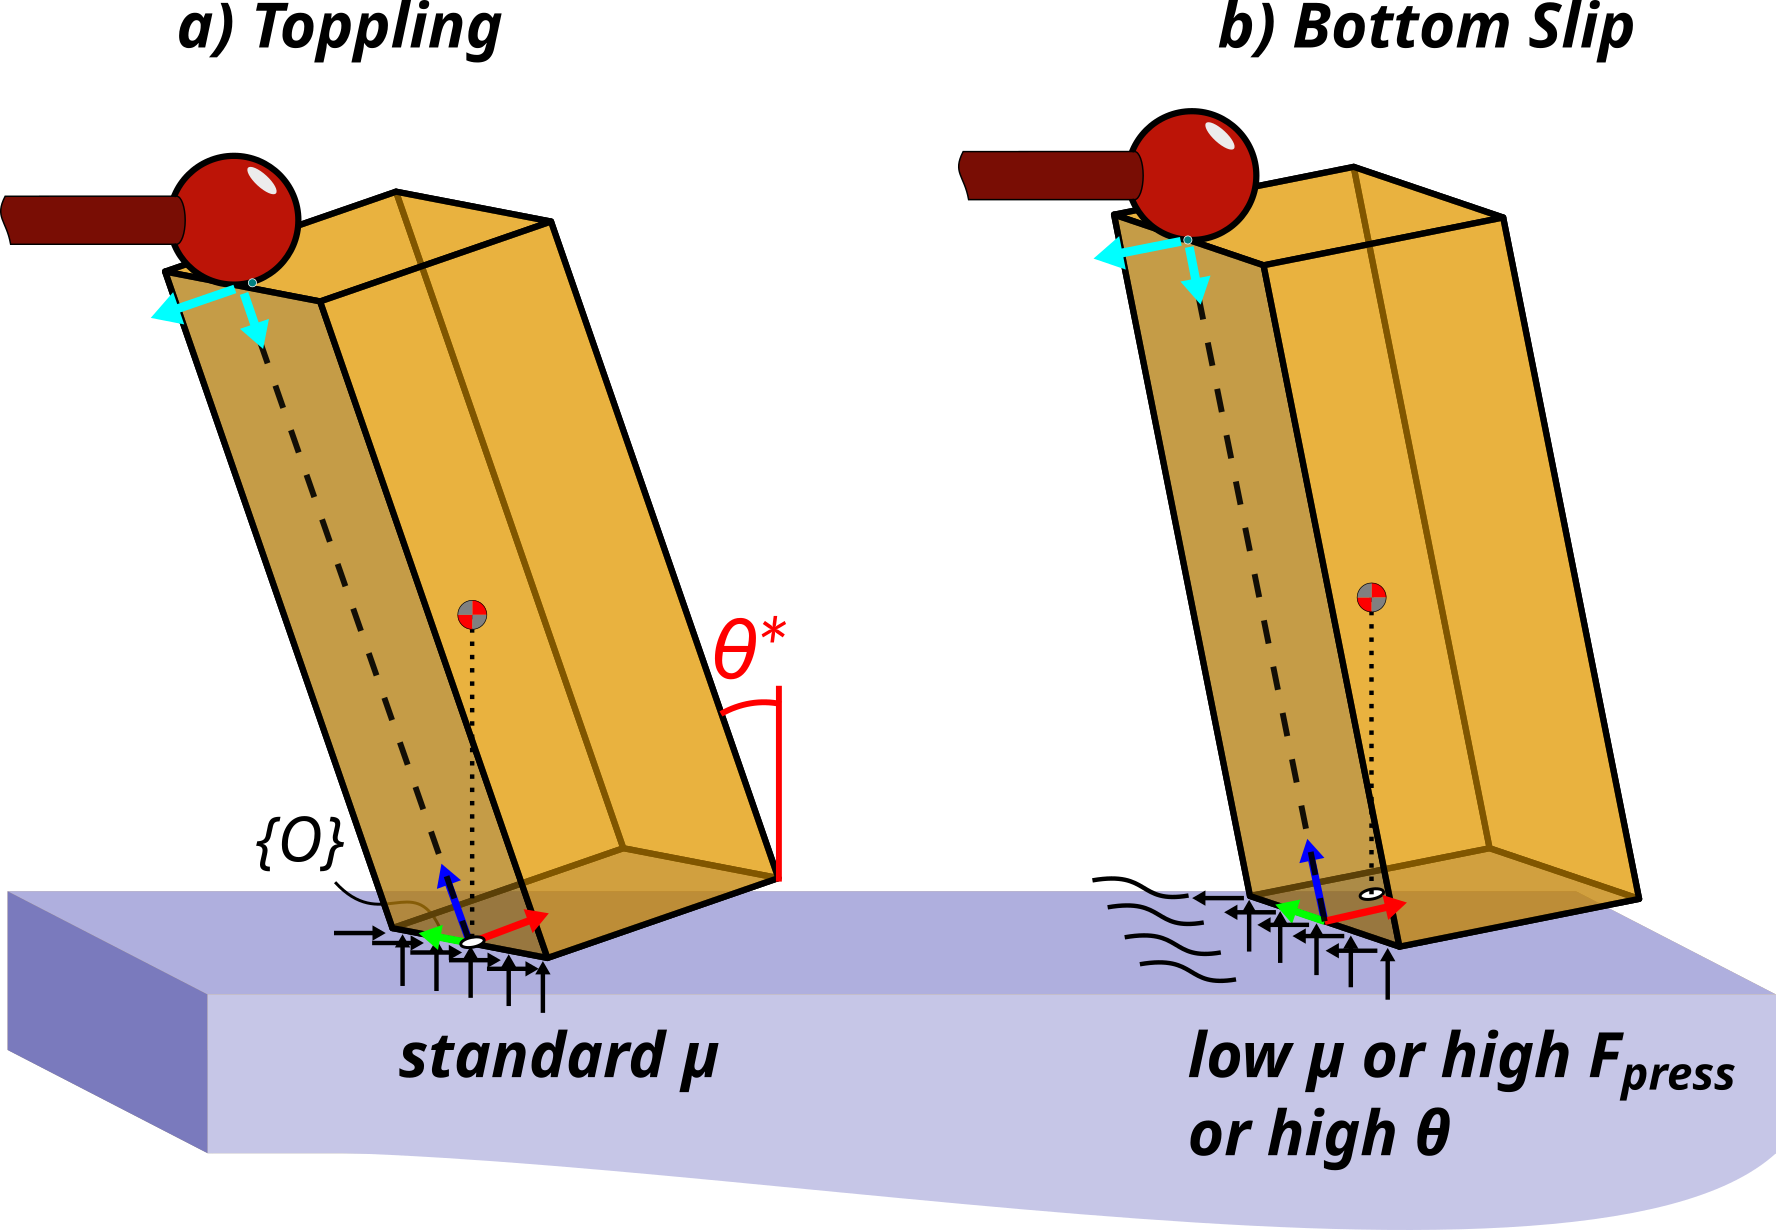
\includegraphics[width=0.95\linewidth]{figures/safety_cases.png}
  \caption{Press-and-pull tipping. A downward press $F_{\mathrm{press}}$ raises the table normal force and pins the pivot, while a pull $F_{\mathrm{pull}}$ tips the object about the near edge through angle $\theta$. As $\theta$ grows, the maintained press acquires a world-horizontal component that adds to the tangential load $f_t$ at the table contact --- the governing hazard. The pull required to sustain quasistatic tipping decays toward zero and crosses it at the toppling angle $\theta^{*}$, beyond which continuing requires the load to reverse into a hold-back force; this sign flip is safe for as long as $f_t$ stays inside the friction cone.}
  \label{fig:hazards}
\end{figure}

This paper closes that gap. Our contributions are:

\begin{itemize}
  \item \textbf{A criticality-aware safety framework that collapses two apparent hazards into one.} We show toppling is a consequence of slip at the object's two passive-grasp contacts rather than an independent hazard, so a single margin
  $\eta_{\mathrm{safety}}$ over the table-slip constraint certifies the whole arc. The press is doubly implicated in this single constraint: increasing it improves early pinning and tipping feasibility but tightens the slip constraint late in the
  arc, so the safe set is a constrained trajectory problem rather than a fixed threshold, and there exists a bounded band of press forces that are simultaneously tipping-feasible and slip-safe.
  
  \item \textbf{A parameter-gated dynamic shove showing the estimates are  \emph{actionable}.} We close the loop on a \emph{shove-to-region} task that is  infeasible without all three parameters, deriving a closed-form admissible push-height window and coast-phase feasibility gate, showing a single dimensionless intensity $\sigma = F/\mu_t m g = D/d_{\mathrm{push}}$ governs the speed--safety tradeoff, and converting the estimator's error bounds into  guaranteed task tolerances --- so the cost of unknown parameters is a predicted, mechanically distinct failure rather than a silent loss of accuracy
  (Section~\ref{sec:validation}).
  
  \item \textbf{Shape-agnostic validation with controlled sweeps.} Beyond an expanded and more irregular object set, we isolate individual claims with parametric sweeps over CoM position, base fillet radius, and pivot geometry, exploring where and how the method degrades.
\end{itemize}

A single design principle spans both sides of the interaction: the running estimation covariance is propagated into both certified margins --- $\eta_{\mathrm{safety}}$ for the probing interaction (Section~\ref{sec:method}) and its shove-side counterpart $\eta_{\mathrm{shove}}$ (Section~\ref{sec:validation}) --- so the estimation and the task it enables both grow more conservative exactly when the parameter estimate is least certain.

The press-and-pull primitive and the multi-modal $(m, z_c, \mu_t)$ decomposition are carried from our prior work \cite{hyland_isrr} and recapped in Section~\ref{sec:background} for self-containment; they are not claimed as new here. We situate the framework against forward tipping, multi-tip equi-effect estimation, and visual/learned methods qualitatively (Table~\ref{tab:method_comparison}), and quantitatively ablate the safety framework itself: the reactive press loop of \cite{hyland_isrr} versus the predictive certification of Section~\ref{sec:method}, on identical objects at matched safety margins (Section~\ref{sec:experiments}).

%% ============================================== 
%% PRIOR WORK 
%% ============================================== 
\section{Prior Work}

\noindent \textbf{Inertial parameter estimation through interaction} Identifying inertial parameters by exciting an object and observing the resulting wrench has a long history, from rigid-body identification of manipulator payloads to in-hand estimation of grasped objects \cite{kubus_-line_2007, sundaralingam_-hand_2021}. Mavrakis and Stolkin \cite{mavrakis_estimation_2020} survey the space along contact model, sensing modality, and active-versus-passive estimation. Most of this work assumes a secure grasp, which excludes precisely the objects that motivate non-prehensile manipulation. Our framework treats the object--table contact not as something to be eliminated by grasping but as a \emph{passive grasp} in the wrench balance.

\noindent \textbf{Pushing-based estimation} Quasistatic planar pushing is a well-studied primitive \cite{mason_mechanics_1986, bauza_probabilistic_2017}. A recurring finding is that planar interaction alone cannot disentangle mass from friction: a small number of pushes fixes only their product, leaving a distribution over both \cite{bauza_probabilistic_2017}. Some methods sidestep identification by closing the loop on force feedback \cite{heins_force_2024}; others recover full parameter sets but require learned interaction models \cite{dutta_push_2023}. Our approach is complementary in spirit but distinct in mechanism: rather than disentangle $m$ and $\mu_t$ within one quasistatic mode, we activate modes sequentially so each reveals the parameters it is suited for.

\noindent \textbf{Friction estimation and slip onset} Friction has classically been estimated through sliding, lateral pressing with tactile sensing, or slip-detection control on grasped objects \cite{sundaralingam_-hand_2021}, with proprioceptive ground-reaction methods used for terrain friction in legged systems \cite{kim_online_2025}, and by observing the resultant motion of pushed objects \cite{lynch_estimating_1993}. We adopt the slip-onset principle but transpose it to a non-prehensile setting, reading friction from the table reaction at incipient slide.

\noindent \textbf{Tipping and toppling} Tipping has been studied both as a manipulation goal and as an estimation tool. Equi-effect methods recover CoM by tipping an object about several axes and intersecting the resulting planes \cite{yong_yu_estimation_1999}, later extended to round-base objects \cite{yong_yu_estimation_2001}; both require multiple interactions and prior knowledge of object geometry, and neither recovers friction. Force-guided single-interaction tipping removes the geometry requirement and the need for repeated tips \cite{hyland_arxiv_tipping}, but fails on low-friction curved bases which slide or swirl before they tip. Our framework retains the benefits of this geometry-free approach, requiring only a single tipping interaction preceded by one planar slide, while resolving its failure mode through the press, treats the resulting press-induced slip as a first-class safety problem, and shows the traditional toppling boundary is a consequence of that same slip constraint rather than an independent hazard.

\noindent \textbf{Safety and uncertainty in non-prehensile manipulation} A separate line of work addresses safety at \emph{execution} time. Robust non-prehensile transport plans against bounded inertial uncertainty rather than estimating it \cite{heins_robust_2025}; model-predictive contact controllers respect friction-cone and non-sliding limits \cite{selvaggio_non-prehensile_2023, heins_keep_2023}; and belief-space planar pushing propagates configuration uncertainty through quasistatic contact dynamics \cite{jankowski_robust_2025}. Classical tip-over stability margins serve the same purpose, from the zero-moment point and the force--angle measure \cite{papadopoulos_rey_1996} to mobile-manipulator descendants such as the moment-height measure \cite{moosavian_alipour_2006}, as does more recent topple-avoiding pushing, whether learned via constrained reinforcement learning \todo{cite: constrained-RL topple-avoiding pushing} or tuned via Bayesian optimization \todo{cite: BO stable pushing}. All of the above certify \emph{execution} of a known plan on a (partially) known object. Our concern is instead safety at \emph{estimation} time: certifying the probing interaction that produces the knowledge in the first place, with the margin computed online from the very quantities being estimated. To our knowledge, safety has not been formalized for non-prehensile inertial estimation in this way.

\noindent \textbf{Positioning} Our work is most closely related to the press-and-pull foundation \cite{hyland_isrr} and to multi-tip equi-effect estimation \cite{yong_yu_estimation_1999, yong_yu_estimation_2001}, with the key difference that we certify the interaction against press-induced object--table slippage in advance, across a single tipping interaction preceded by one planar slide, show the toppling boundary is a consequence of that same slip constraint rather than an independent hazard, and characterize the resulting safety--accuracy tradeoff, including the benefit of crossing the toppling angle when an object's slip budget allows it. The downstream shove-to-region validation of Section \ref{sec:validation} is likewise adjacent to, but distinct from, the classical pushing literature: quasistatic stable pushing \cite{mason_mechanics_1986} and the differentially-flat pusher--slider line \cite{zhou_pushing_nodate} are planar and controllability/planning-focused rather than tipping-aware, and robust nonprehensile transport \cite{heins_robust_2025} plans \emph{around} bounded inertial uncertainty rather than consuming an online estimate. We are not aware of a closed-form admissible push-height window for a dynamic, released shove expressed directly in the estimated parameters, nor of the dimensionless shove-intensity identity of Section \ref{sec:validation}; the underlying tipping mechanics are classical, and our contribution is assembling them into a parameter-gated feasibility certificate rather than a new pushing theory.

%% ============================================== 
%% Background 
%% ============================================== 
\section{Background} \label{sec:background}

This section recaps the forward-tipping and press-and-pull models from \sh{IROS, ISRR} to the extent needed for the safety analysis in Section \ref{sec:method}. We assume throughout a non-deformable rigid body, quasistatic motion (for estimation), and a single isotropic Coulomb friction coefficient $\mu_t$ at the object--table contact.

\paragraph{Forward tipping}
Let $\{O\}$ be the object frame located on the pivot edge and $\theta$ the object's out-of-plane rotation about that edge. At a fixed pivot the quasistatic torque balance
\begin{equation}
    {}^{O}\mathbf{p}_{\mathrm{push}}\times{}^{O}\mathbf{F}_{\mathrm{push}}
    + {}^{O}\mathbf{p}_{c}\times{}^{O}\mathbf{F}_{\mathrm{grav}} = \mathbf{0}
    \label{eq:torque_balance}
\end{equation}
recovers $(m, z_c)$, with $\mu_t$ structurally absent: tipping is friction-agnostic by construction. Whether an object tips at all is decided by the competing onset thresholds
\begin{equation}
  ||\mathbf{F}_\mathrm{push}|| = \;  
  F_{\mathrm{slide}} = \mu_t N, \qquad
    F_{\mathrm{tip}} = \frac{\lVert \mathbf{p}_c\times\mathbf{F}_{\mathrm{grav}}\rVert}
                            {\lVert\mathbf{p}_{\mathrm{push}}\rVert \sin\alpha},
    \label{eq:thresholds}
\end{equation}
where $\alpha$ is the angle between the applied force and the tip direction. Forward tipping is infeasible when $F_{\mathrm{slide}} < F_{\mathrm{tip}}$ for all admissible push heights, which is exactly the low-friction / smooth-base regime.

\paragraph{Press-and-pull}
The press-and-pull primitive drives the ordering $F_{\mathrm{tip}} < F_{\mathrm{slide}}$ by raising $F_{\mathrm{slide}}$ directly. A downward press of magnitude $F_{\mathrm{press}}$ raises the table normal force to $N = mg + F_{\mathrm{press}}$ and the sliding threshold to $F_{\mathrm{slide}} = \mu_t(mg + F_{\mathrm{press}})$, while a horizontal pull drives tipping about the near pivot edge (Fig. \ref{fig:hazards}). The press uses the object's own support surface as a passive grasp, pinning the pivot through frictional engagement and allowing curved-edge and low-friction bases to tip rather than slide or swirl. The full measured wrench is mapped to the object, ${}^{O}\mathbf{w}_\mathrm{app}$, by the adjoint transform
\begin{equation}
    {}^{O}\mathbf{w}_{\mathrm{app}} = -\,\mathrm{Ad}^{\!\top}_{T_{SO}}\,{}^{S}\mathbf{w}_{\mathrm{meas}},
    \label{eq:adjoint}
\end{equation}
using only the proprioceptive sensor pose $T_{SO}$ and bypassing error-prone contact-point localization.

\paragraph{Multi-modal decomposition} A planar slide observes the coupled product $\mu_t m$ at slip onset; press-and-pull tipping recovers $m$ from the same friction-free torque balance as \eqref{eq:torque_balance}, now taken about the pivot over the \emph{total} applied wrench of \eqref{eq:adjoint}. The press contributes a moment about the pivot as well as the pull, but table friction is structurally absent from the balance either way, so the balance remains friction-free even though it is no longer single-force; friction then follows in closed form as $\mu_t = (\mu_t m)/m$, with no second sliding interaction (Fig. \ref{fig:pipeline}).

\begin{figure}[t]
  \centering
  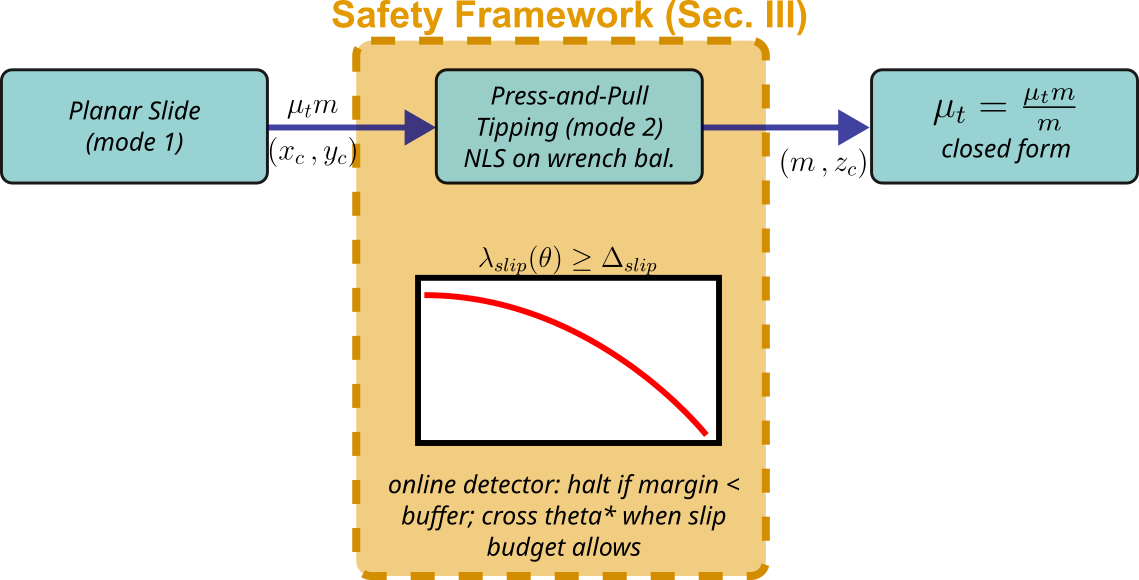
\includegraphics[width=0.95\linewidth]{figures/pipeline.png}
  \caption{Multi-modal pipeline. A planar slide caches the product $\mu_t m$ and supplies planar CoM $(x_c, y_c)$; press-and-pull tipping recovers $(m, z_c)$ via nonlinear least squares on the wrench balance; friction is then recovered in closed form. The safety framework of Section \ref{sec:method} wraps the tipping interaction. \sh{PLACEHOLDER}.}
  \label{fig:pipeline}
\end{figure}

%% ============================================== 
%% Methodology 
%% ============================================== 
\section{Methodology} \label{sec:method}

The estimation interaction must drive the object far enough up the tipping arc to observe the parameters cleanly, without letting either of its two passive-grasp contacts slip. We first show why toppling is a consequence of that slip rather than an independent hazard, then derive the coupling between the press and the table-slip constraint, then define the admissible interaction set and a single margin that certifies the whole arc, and finally describe the online detector, the safety--accuracy tradeoff, and an optional covariance coupling.

\subsection{Problem setup} We analyze the tipping motion in the vertical plane containing the pull direction and the pivot, parameterized by the object angle $\theta \in [0, \theta_{\mathrm{end}}]$, where $\theta_{\mathrm{end}}$ is set below by the slip margin rather than fixed a priori. $\theta^{*}$ denotes the \emph{toppling angle} at which the CoM passes over the pivot; it is a waypoint the arc may or may not cross, not a boundary on $\theta_{\mathrm{end}}$. The press force is maintained along the object's top-face normal $\hat{\mathbf{n}}(\theta)$ throughout the motion. Observing Figure \ref{fig:zoom}, control is applied in this finger-fixed frame: $F_{\mathrm{press}}$ is a regulated normal force held throughout the arc, while the pull is a velocity command along $\hat{\mathbf{t}}(\theta)$ and $F_{\mathrm{pull}}(\theta)$ denotes the resulting signed tangential component (not world-frame vertical/horizontal quantities). Eqs.~\eqref{eq:Nt}--\eqref{eq:ft} below project these onto the world vertical and horizontal at the table contact, and because the pull is kinematic, $F_{\mathrm{pull}}$ reverses sign on its own as the object crosses $\theta^{*}$---no force-switching logic is needed and the equations hold unchanged across the crossing. The object--table contact supports a normal force $N_t(\theta)$ and a tangential reaction $f_t(\theta)$ that must remain within the friction cone.

\subsection{Two contacts, one governing hazard}
The press-and-pull primitive maintains two passive-grasp contacts throughout the arc: the finger against the object's top face, and the object's base against the table. As long as neither contact slips, the object is kinematically locked to the commanded pivot rotation and cannot fall over on its own. An uncontrolled topple is only possible if both constraints are broken by a slip at either of the two contact interfaces. Toppling is therefore only a consequence of a prior slip, and bounding the friction-cone margin at both contacts is sufficient to prevent it. 

In this paper we hold the finger-object contact by design with a rigid, high-friction fingertip pressed with sufficient force. The one hazard we dynamically certify is therefore how close the table contact is to slipping (the \emph{slip margin}); we additionally track proximity to the toppling angle (the \emph{toppling margin}) as a diagnostic, not as a second constraint, since it is not itself an independent failure mode. The finger contact, while not certified online, is not left unchecked: its friction-cone margin follows from the same measured wrench \eqref{eq:adjoint}, and we report it in Section \ref{sec:results} to verify the design assumption holds in practice.

\noindent \textbf{Toppling}
At $\theta^{*}$ the gravitational moment about the pivot changes sign: below it, gravity restores the object and sustaining quasistatic rotation requires an outward pull; beyond it, gravity itself continues the rotation, so sustaining a controlled increase in $\theta$ requires the applied load to reverse into a hold-back force. Because the object remains kinematically locked to the arc as long as neither passive-grasp contact slips, this sign flip is not itself a fall, it is safe for as long as the (now reversed) load stays inside the table-slip margin. We track it with the \emph{toppling margin}
\begin{equation}
    \lambda_{\mathrm{topple}}(\theta) = \frac{F_{\mathrm{pull}}^{\mathrm{meas}}(\theta)}{F_{\mathrm{pull}}^{\mathrm{peak}}}
    \;\in\;(-\infty,1],
    \label{eq:m_topple}
\end{equation}
which is near $1$ early in the arc, crosses zero exactly at $\theta^{*}$, and continues negative beyond it as the hold-back load grows. Here $F_{\mathrm{pull}}^{\mathrm{peak}} \triangleq F_{\mathrm{pull}}(\theta \to 0)$, the pull required at the start of the arc. Because the required pull decays monotonically with $\theta$, this starting value is also the maximum over the arc; normalizing by it, rather than by a running maximum, fixes the normalizer at the onset of the pull, so $\lambda_{\mathrm{topple}}$ is evaluable for the remainder of the arc from the first instants of interaction. Whether an arc can cross $\theta^{*}$ is decided entirely by the slip margin, not by $\lambda_{\mathrm{topple}}$ itself. Crossing is preferred when available: it replaces an asymptotic extrapolation with a direct zero-crossing observation, sharpening $z_c$.

\noindent \textbf{Object-table slippage}
The press-and-pull primitive introduces a hazard absent from forward tipping. The table contact slips when the tangential reaction reaches the friction limit,
\begin{equation}
    \lVert f_t(\theta)\rVert \;=\; \mu_t\, N_t(\theta).
    \label{eq:slip_condition}
\end{equation}
Figure \ref{fig:zoom} shows the setup above, where the dominant contributions to the normal and tangential balances are
\begin{align}
    N_t(\theta) &\approx mg + F_{\mathrm{press}}\cos\theta + F_{\mathrm{pull}}(\theta)\sin\theta, \label{eq:Nt}\\
    \lVert f_t(\theta)\rVert &\approx F_{\mathrm{pull}}(\theta)\cos\theta + F_{\mathrm{press}}\sin\theta,
    \label{eq:ft}
\end{align}
where the $\cos\theta$ and $\sin\theta$ terms are the projections of the maintained press and pull forces onto the world vertical and horizontal as the press-face normal rotates with $\theta$. The $\approx$ neglects second-order terms from the finite contact-patch size at the pivot, consistent with the point-pivot, single-contact rigid-body assumptions of Section \ref{sec:method}. This term remains small under the press magnitudes and finger geometry used here.

\begin{figure}[t]
  \centering
  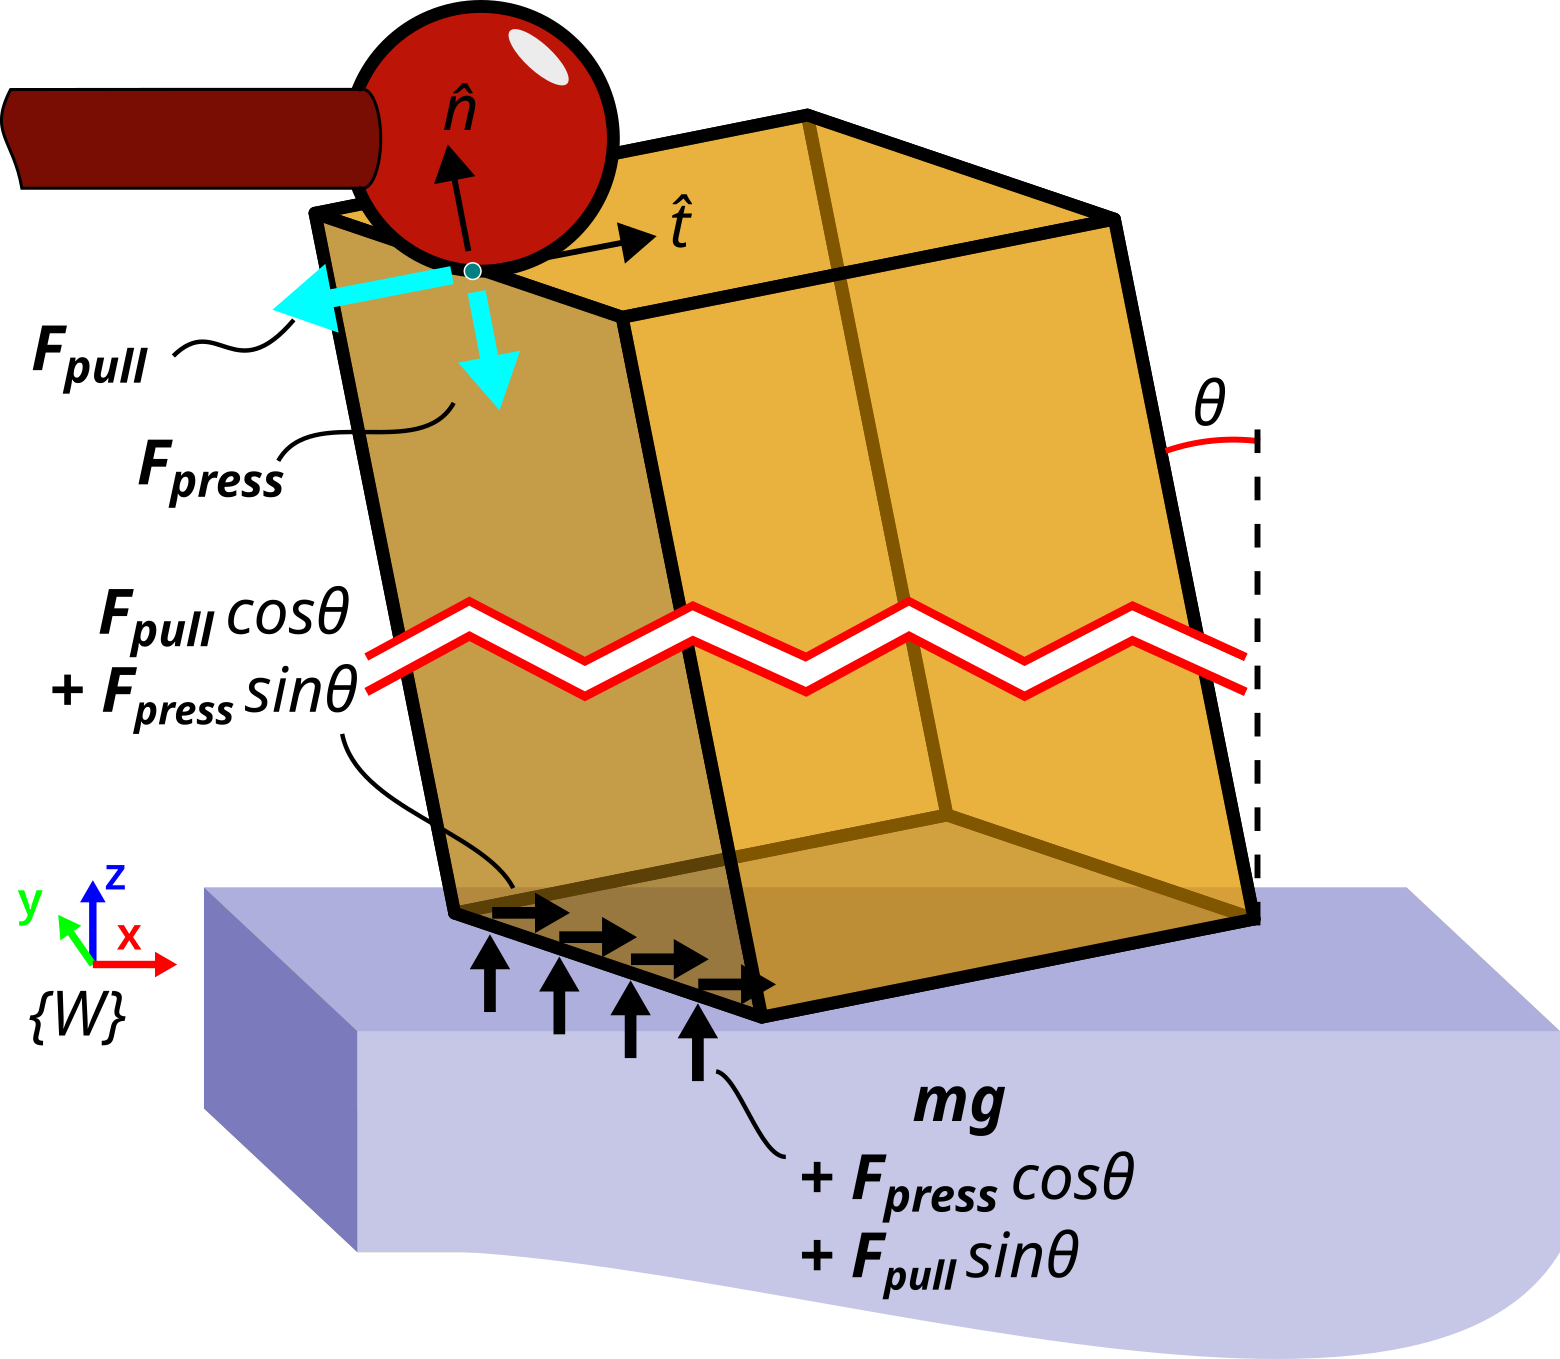
\includegraphics[width=0.95\linewidth]{figures/zoom.png}
  \caption{Zoomed-in view of the normal and tangential balances for the slip margin.\sh{Show friction cone in this figure?}}
  \label{fig:zoom}
\end{figure}


The corresponding \emph{slip margin} is the normalized friction-cone slack,
\begin{equation}
    \lambda_{\mathrm{slip}}(\theta)
    = 1 - \frac{\lVert f_t(\theta)\rVert}{\mu_t\, N_t(\theta)}
    \;\in\;(-\infty, 1],
    \label{eq:m_slip}
\end{equation}
positive inside the cone and zero at incipient slip.

% \subsection{The coupling and the safe press band}
% Equations \eqref{eq:Nt}--\eqref{eq:ft} expose the central structural fact of the press-and-pull primitive: the press force enters both the normal and tangential balances, with opposite effect on the slip margin as $\theta$ grows. Early in the arc ($\theta$ small), $\cos\theta\approx 1$ and $\sin\theta\approx 0$, so raising $F_{\mathrm{press}}$ raises $N_t$ and improves $\lambda_{\mathrm{slip}}$. Therefore, a sufficiently large press is what makes the object tip rather than slide at all (\eqref{eq:thresholds}). Late in the arc, $\sin\theta$ grows and the $F_{\mathrm{press}}\sin\theta$ term inflates the tangential load faster than $\cos\theta$ sustains the normal force, so the \emph{same} press now erodes $\lambda_{\mathrm{slip}}$. 

% The practical consequence is that a larger press is \emph{not} uniformly safer, contrary to the intuition that the press only stabilizes. For a given object there is a bounded
% \emph{safe press band}

% \begin{equation*}
%     \mathcal{F}_{\mathrm{press}} = \left[\, \underline{F},\; \overline{F} \,\right], 
% \end{equation*}
% \begin{equation}
%     \quad \underbrace{F_{\mathrm{tip}} < \mu_t (mg + \underline{F})}_{\text{tipping feasible}}, \quad \underbrace{\lambda_{\mathrm{slip}}(\theta) \geq 0 \;\; \forall \theta \;\text{at}\; \overline{F}}_{\text{no late-arc slip}}
% \end{equation}

% whose lower bound is set by tipping feasibility and whose upper bound is set by late-arc slip. The adaptive press loop of \cite{hyland_isrr} searched for \emph{a} point inside $\mathcal{F}_{\mathrm{press}}$ reactively, increasing the press after observing a failed arc; the framework here makes the band itself the object of reasoning and the margin predictive.

% The band also generalizes beyond a single constant $F_{\mathrm{press}}$. Eqs.~\eqref{eq:Nt}--\eqref{eq:ft} define $\lambda_{\mathrm{slip}}(\theta)$ for any press \emph{schedule} $F_{\mathrm{press}}(\theta)$, not only a constant one, so the margin-preserving schedule is the one satisfying $\lambda_{\mathrm{slip}}(\theta) \equiv \Delta_{\mathrm{slip}}$ once a constant press would dip below it: hold the pinning press early in the arc, where it is needed for tipping feasibility, and taper it late in the arc, where it erodes the margin. The safe press \emph{band} therefore generalizes to a safe press \emph{tube} $F_{\mathrm{press}}(\theta)$, and the certified margin is itself the feedforward law for that tube. We use a constant press in the experiments of Section \ref{sec:results} and leave the closed-loop press schedule to future work (Section \ref{sec:conclusion}), but note it directly here since it answers, within the same framework, whether overall force should decrease at larger tip angles.

% \subsection{Admissible interaction set and unified safety margin}

% An interaction is specified by a press force $F_{\mathrm{press}}$ and an arc terminating at $\theta_{\mathrm{end}}$, which is \emph{not} constrained to lie below $\theta^{*}$: since toppling is a consequence of slip rather than an independent hazard, the arc may cross the toppling angle whenever the table contact can sustain it. We require the slip margin be respected with a prescribed buffer $\Delta_{\mathrm{slip}} \in (0,1)$ across the entire executed arc, and define the admissible set
% \begin{equation}
%     \mathcal{A} = \big\{ (F_{\mathrm{press}}, \theta_{\mathrm{end}}) :
%         \lambda_{\mathrm{slip}}(\theta) \ge \Delta_{\mathrm{slip}},
%         \ \forall\theta \in [0,\theta_{\mathrm{end}}] \big\}.
%     \label{eq:admissible}
% \end{equation}
% A single scalar certifies a candidate interaction by reporting its worst-case proximity to the table-slip hazard over the whole arc:
% \begin{equation}
%     \eta_{\mathrm{safety}}
%     = \min_{\theta \in [0,\theta_{\mathrm{end}}]} \lambda_{\mathrm{slip}}(\theta).
%     \label{eq:eta}
% \end{equation}
% The interaction is admissible iff $\eta_{\mathrm{safety}} \ge \Delta_{\mathrm{slip}}$. The toppling margin $\lambda_{\mathrm{topple}}$ is deliberately absent from this certification: it is retained as a diagnostic that locates the sign flip at $\theta^{*}$ (Eq. \eqref{eq:m_topple} crosses zero there), useful for anticipating the load reversal and for reading $\theta^{*}$ directly off the data when the arc extends past it. The fixed sub-critical pull-fraction cutoff of prior work \cite{hyland_isrr, hyland_arxiv_tipping} --- halting whenever $\lambda_{\mathrm{topple}}$ fell below a constant threshold --- is recovered here only as one conservative choice of $\theta_{\mathrm{end}}$, one that never approaches $\theta^{*}$; this paper's claim is that fixing $\theta_{\mathrm{end}}$ that way is not required by safety, only by the older primitive's inability to reverse its own applied load.

\subsection{The coupling and the safe press band}
Equations \eqref{eq:Nt}--\eqref{eq:ft} expose the central structural fact of the press-and-pull primitive: the press force enters both the normal and tangential balances, with opposite effect on the slip margin as $\theta$ grows. Early in the arc ($\theta$ small), $\cos\theta\approx 1$ and $\sin\theta\approx 0$, so raising $F_{\mathrm{press}}$ raises $N_t$ and improves $\lambda_{\mathrm{slip}}$. Therefore, a sufficiently large press is what makes the object tip rather than slide at all (Eq.~\eqref{eq:thresholds}). Late in the arc, $\sin\theta$ grows and the $F_{\mathrm{press}}\sin\theta$ term inflates the tangential load faster than $\cos\theta$ sustains the normal force, so the \emph{same} press now erodes $\lambda_{\mathrm{slip}}$.

The practical consequence is that a larger press is \emph{not} uniformly safer, contrary to the intuition that the press only stabilizes. For a given object there is a bounded \emph{safe press band}
\begin{equation*}
    \mathcal{F}_{\mathrm{press}} = \left[\, \underline{F},\; \overline{F} \,\right],
\end{equation*}
\begin{equation}
    \quad \underbrace{F_{\mathrm{tip}} < \mu_t (mg + \underline{F})}_{\text{tipping feasible}}, \quad \underbrace{\lambda_{\mathrm{slip}}(\theta) \geq 0 \;\; \forall \theta \;\text{at}\; \overline{F}}_{\text{no late-arc slip}}
\end{equation}
whose lower bound is set by tipping feasibility and whose upper bound is set by late-arc slip. The adaptive press loop of \sh{ISRR} searched for \emph{a} point inside $\mathcal{F}_{\mathrm{press}}$ by retrying: increasing the press only after observing a completed failed arc. The band's limits are not knowable before contact, they depend on the very $(m, \mu_t)$ being estimated, but once the slide mode has cached $\mu_t m$ and $m$ stabilizes in the first portion of the pull, the margin trajectory for the \emph{remainder} of the arc follows from \eqref{eq:Nt}--\eqref{eq:ft}: reasoning about the band begins moments into an interaction rather than one failed arc after it.

The band also generalizes beyond a single constant $F_{\mathrm{press}}$. Eqs.~\eqref{eq:Nt}--\eqref{eq:ft} define $\lambda_{\mathrm{slip}}(\theta)$ for any press \emph{schedule} $F_{\mathrm{press}}(\theta)$, not only a constant one: at each $\theta$ the constraints admit a press interval, and these intervals stacked along the arc form a \emph{tube} in the $(\theta, F_{\mathrm{press}})$ plane that any admissible schedule must thread, with a constant press the special case of a horizontal line inside it. The margin-preserving schedule holds the pinning press early in the arc, where it is needed for tipping feasibility, and tapers it late in the arc to satisfy $\lambda_{\mathrm{slip}}(\theta) \equiv \Delta_{\mathrm{slip}}$, where $\Delta_{\mathrm{slip}} \in (0,1)$ is a prescribed buffer of friction-cone slack retained at all times; the certified margin is itself the feedforward law for that tube. In Section \ref{sec:results} we use a constant press for the parametric sweeps, so that each sweep varies a single factor and the framework's contribution is not conflated with press scheduling, and demonstrate the tapered schedule separately on objects whose band admits no constant press over the full arc. \sh{This is to say we will keep Fpress constant for estimation. Except for some objects where keeping Fpress is not enough for good accuracy, then we do adaptive press force during the tip.}

\subsection{Admissible interaction set and unified safety margin}

An interaction is specified by a press force $F_{\mathrm{press}}$ and an arc terminating at $\theta_{\mathrm{end}}$, which is \emph{not} constrained to lie below $\theta^{*}$: since toppling is a consequence of slip rather than an independent hazard, the arc may cross the toppling angle whenever the table contact can sustain it. A single scalar certifies a candidate interaction by reporting its worst-case proximity to the table-slip hazard over the whole arc:
\begin{equation}
    \eta_{\mathrm{safety}}
    = \min_{\theta \in [0,\theta_{\mathrm{end}}]} \lambda_{\mathrm{slip}}(\theta).
    \label{eq:eta}
\end{equation}
An interaction is admissible iff $\eta_{\mathrm{safety}} \ge \Delta_{\mathrm{slip}}$, and the admissible set $\mathcal{A} = \{ (F_{\mathrm{press}}, \theta_{\mathrm{end}}) : \eta_{\mathrm{safety}} \ge \Delta_{\mathrm{slip}} \}$ collects the certified designs. The toppling margin $\lambda_{\mathrm{topple}}$ is deliberately absent from this certification: it is retained as a diagnostic that locates the sign flip at $\theta^{*}$ (Eq.~\eqref{eq:m_topple} crosses zero there), useful for anticipating the load reversal and for reading $\theta^{*}$ directly off the data when the arc extends past it. The fixed sub-critical pull-fraction cutoff of prior work \sh{ISRR, IROS} --- halting whenever $\lambda_{\mathrm{topple}}$ fell below a constant threshold --- is recovered here only as one conservative choice of $\theta_{\mathrm{end}}$, one that never approaches $\theta^{*}$; this paper's claim is that fixing $\theta_{\mathrm{end}}$ that way is not required by safety, only by the older primitive's inability to reverse its own applied load.

\subsection{Online safety detector}

Every quantity in the slip margin \eqref{eq:m_slip} is available online: the adjoint transform \eqref{eq:adjoint} gives $N_t(\theta)$ and $f_t(\theta)$ from the measured wrench, proprioception gives $\theta$ and the pull magnitude, and $\mu_t$ comes from the slide mode. The detector therefore tracks $\eta_{\mathrm{safety}}$ continuously and retracts the arc before the slip margin is breached; $\lambda_{\mathrm{topple}}$ is only logged as a diagnostic, so the arc may pass through $\theta^{*}$ whenever the slip margin permits. Pose deviation from the commanded arc provides an independent geometric slip check.

Because $\mu_t$ and $m$ are known early in the pull, the detector is predictive: from \eqref{eq:Nt}--\eqref{eq:m_slip} it projects the slip-margin trajectory $\lambda_{\mathrm{slip}}(\theta)$ over the remaining arc before traversing it, rather than reacting at the onset of slip.

\subsection{Safety--accuracy tradeoff}

The same proximity that creates risk creates information, and the risk is now singular: it is the slip buffer $\Delta_{\mathrm{slip}}$, not a separate toppling buffer, that trades against accuracy. The CoM height $z_c$ is most sharply fixed by directly observing the sign flip of $F_{\mathrm{pull}}(\theta)$ at $\theta^{*}$; whether an arc's slip budget extends far enough to reach and cross $\theta^{*}$ depends on the object ($\mu_t$, mass, chosen press) and is read from the predicted slip limit. A generous $\Delta_{\mathrm{slip}}$ stops well short of the slip limit and, for low-friction or heavily pressed objects, short of $\theta^{*}$ as well, leaving $z_c$ to be inferred from the pre-crossing decay trend alone; a tighter $\Delta_{\mathrm{slip}}$, or a more favorable press, can admit the crossing and its sharper $z_c$ observation, at reduced margin against the one hazard that remains. $m$, observable throughout the arc, is comparatively insensitive to this choice. We characterize this tradeoff empirically in Section \ref{sec:results}.

\subsection{Estimation conditioning and the press band} \label{sec:conditioning}

Beyond tipping feasibility below and slip safety above, a third consideration favors the low end of the press band \eqref{eq:press_band}: estimation conditioning. Fitting $m$ relies on the gravitational moment $mg\,\lVert\mathbf{p}_c\rVert$ about the pivot \eqref{eq:torque_balance}, whose signal-to-noise ratio scales with $m$, so light objects are hardest to estimate (Section \ref{sec:results}). A large press worsens this: since $F_{\mathrm{press}}$ acts through the finger contact rather than the pivot, any lever-arm error injects a spurious moment (that error times $F_{\mathrm{press}}$) onto the same balance, and under a large press it can dominate the pull-torque signal and correlate the recovered $m$ with press magnitude. We therefore bias the press low during the estimation window and quantify the sensitivity in Section \ref{sec:results}.

\subsection{Covariance-coupled margin}

\sh{What I'm thinking for this section:} Inflate the safety-margin threshold $\Delta_{\mathrm{slip}}$ in proportion to the estimation covariance $\Sigma$ from the least-squares fit, so the interaction automatically backs off when $\mu_t,m$ are poorly estimated ($\Delta_{\mathrm{slip}} \leftarrow \Delta_{\mathrm{slip}} + \kappa\,g(\Sigma)$). The appeal is that the same $\Sigma$ also feeds the shove-side gate in Section~\ref{sec:validation}, so it would have been ``one principle applied twice.'' Open question: do we (a) drop it entirely, (b) keep it as a one-line future-work mention in the conclusion, or (c) actually run the experiment to back it?

% Basically, use the uncertainty to determine how far to tip the object. This will be similar to the shove task, whose success depends on accurate estimation of the parameters for determining shove force and height.


% When the parameter estimate is poorly conditioned, as identified above, the nominal margins may be optimistic, since they are evaluated using uncertain $\mu_t$ and $m$. We couple the running estimation covariance $\Sigma$ from the nonlinear least-squares fit into the margin by inflating the thresholds in proportion to the estimate uncertainty,
% \begin{equation}
%     \Delta_{\bullet} \leftarrow \Delta_{\bullet} + \kappa\, g(\Sigma),
%     \label{eq:cov_coupling}
% \end{equation}
% with gain $\kappa$ and a scalar uncertainty summary $g(\Sigma)$ (e.g.\ a trace or a relevant diagonal term), so the interaction backs off automatically when the fit is least trustworthy. This coupling requires no additional hardware or interaction modality, only the covariance already produced by the fit, and it has a direct downstream consumer: the same $\Sigma$ sets the parameter-error terms $\varepsilon_{z_c}, \varepsilon_\mu, \varepsilon_m$ in the shove-side uncertainty gate of Section \ref{sec:validation} (Eq. \eqref{eq:tip_gate}), so tightening $\eta_{\mathrm{safety}}$ under high covariance at estimation time and tightening the required shove margin under that same covariance at task time are one principle applied twice. We present the coupling itself as a design-time principle rather than a separately validated subsystem, and leave its end-to-end empirical validation, together with its use inside a closed-loop controller that selects the press online, to future work (Section \ref{sec:conclusion}).

%% ============================================== 
%% Results 
%% ============================================== 
\section{Experiments, Results, and Discussion} \label{sec:results} 
% NOTE: scaffold + framing only. No invented numbers; [bracketed] placeholders to fill from data. % Qualitative trend statements are written as expectations grounded in the physics / the ISRR % foundation, not as established journal results.

\subsection{Experimental setup} 
We use the hardware of \cite{hyland_isrr}: an ABB IRB120 industrial manipulator, a wrist-mounted ATI Gamma six-axis force/torque sensor sampled at 500\,Hz, an Intel RealSense D435i for object point clouds, and a rigid high-friction spherical finger providing point contact for both modes. The finger is single-contact throughout; a dual-contact ("fork") end-effector is left to future work (Section \ref{sec:conclusion}). The object set (Fig. \ref{fig:lineup}) comprises designed primitives, for which ground truth is exact, and irregular everyday items including a sculpture, for which ground truth is measured independently and treated as approximate.

\begin{figure}[t]
  \centering
  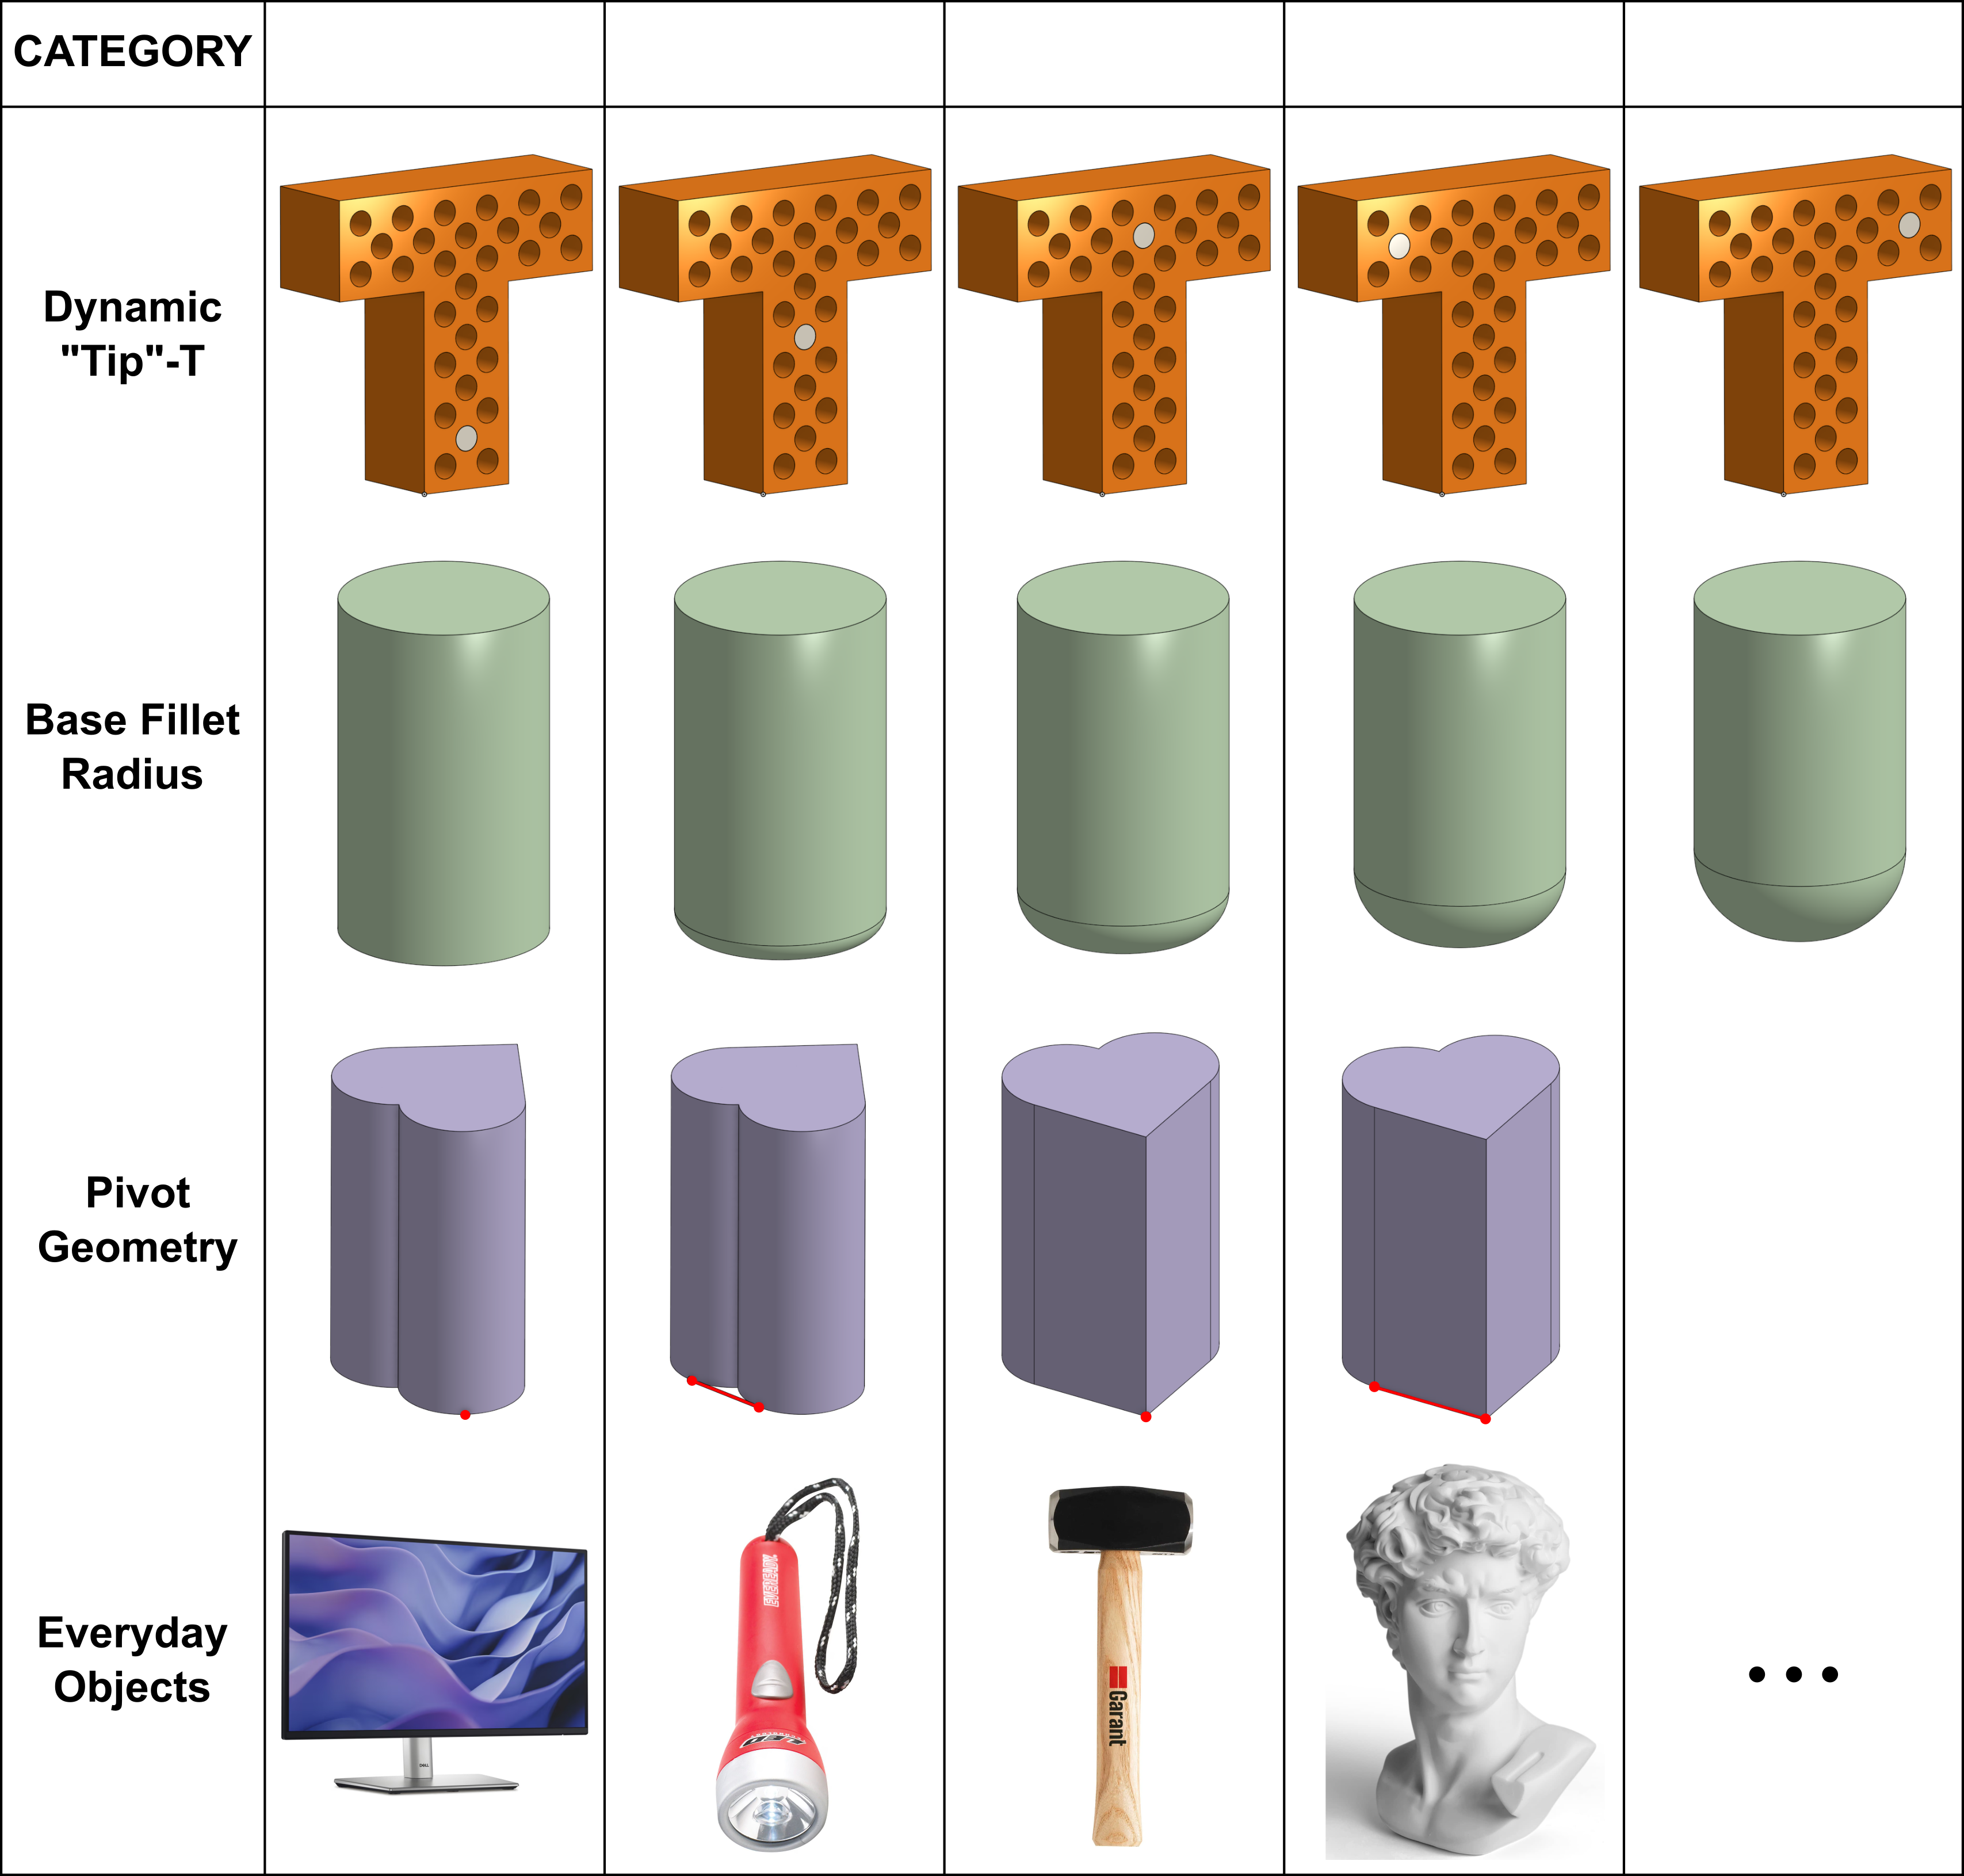
\includegraphics[width=0.95\linewidth]{figures/lineup.png}
  \caption{Object set: designed primitives with exact ground truth, and irregular everyday items with approximate ground truth.}
  \label{fig:lineup}
\end{figure}

\subsection{Multi-modal accuracy} 
Table \ref{tab:results} reports estimated $(m, z_c, \mu_t)$ against ground truth across the full set. \todo{fill table from data.} We expect the heavier objects to yield the cleanest estimates, as a larger gravitational torque produces a higher signal-to-noise wrench trajectory during tipping, and the lightweight wide-smooth-base regime to be hardest, consistent with the conditioning analysis of Section \ref{sec:method}.

\begin{table}[t]
  \centering
  \caption{Estimation results on physical objects (to be completed).}
  \label{tab:results}
  \small
  \begin{tabular}{l ccc ccc}
    \toprule
    & \multicolumn{3}{c}{\textbf{Ground truth}} & \multicolumn{3}{c}{\textbf{Rel.\ error (\%)}} \\
    \cmidrule(lr){2-4}\cmidrule(lr){5-7}
    \textbf{Object} & $m$ & $z_c$ & $\mu_t$ & $|\Delta m|$ & $|\Delta z_c|$ & $|\Delta\mu_t|$ \\
    \midrule
    \todo{fill from data} & [\,] & [\,] & [\,] & [\,] & [\,] & [\,] \\
    $\vdots$ &      &      &      &      &      &      \\
    \bottomrule
  \end{tabular}
\end{table}

\subsection{Controlled parametric sweeps}
Each sweep isolates a single claim:
\begin{itemize}
  \item \textbf{CoM position (Tip-T).} A swappable internal mass translates the CoM along the object; we report estimation error versus CoM offset to test sensitivity across the identifiable range.
  \item \textbf{Base fillet radius.} We sweep the base edge from sharp to fully rounded and report estimation quality versus fillet radius. This maps where the fixed-pivot assumption degrades, rather than claiming arbitrary curved bottoms are solved; we expect graceful degradation up to a radius beyond which the pivot can no longer be pinned.
  \item \textbf{Pivot geometry.} We vary the pivot-edge shape directly to probe the assumption that the pivot is a well-defined line.
\end{itemize}
\todo{Fill Fig. \ref{fig:sweeps} with sweep data.}
\begin{figure}[t]
  \centering
  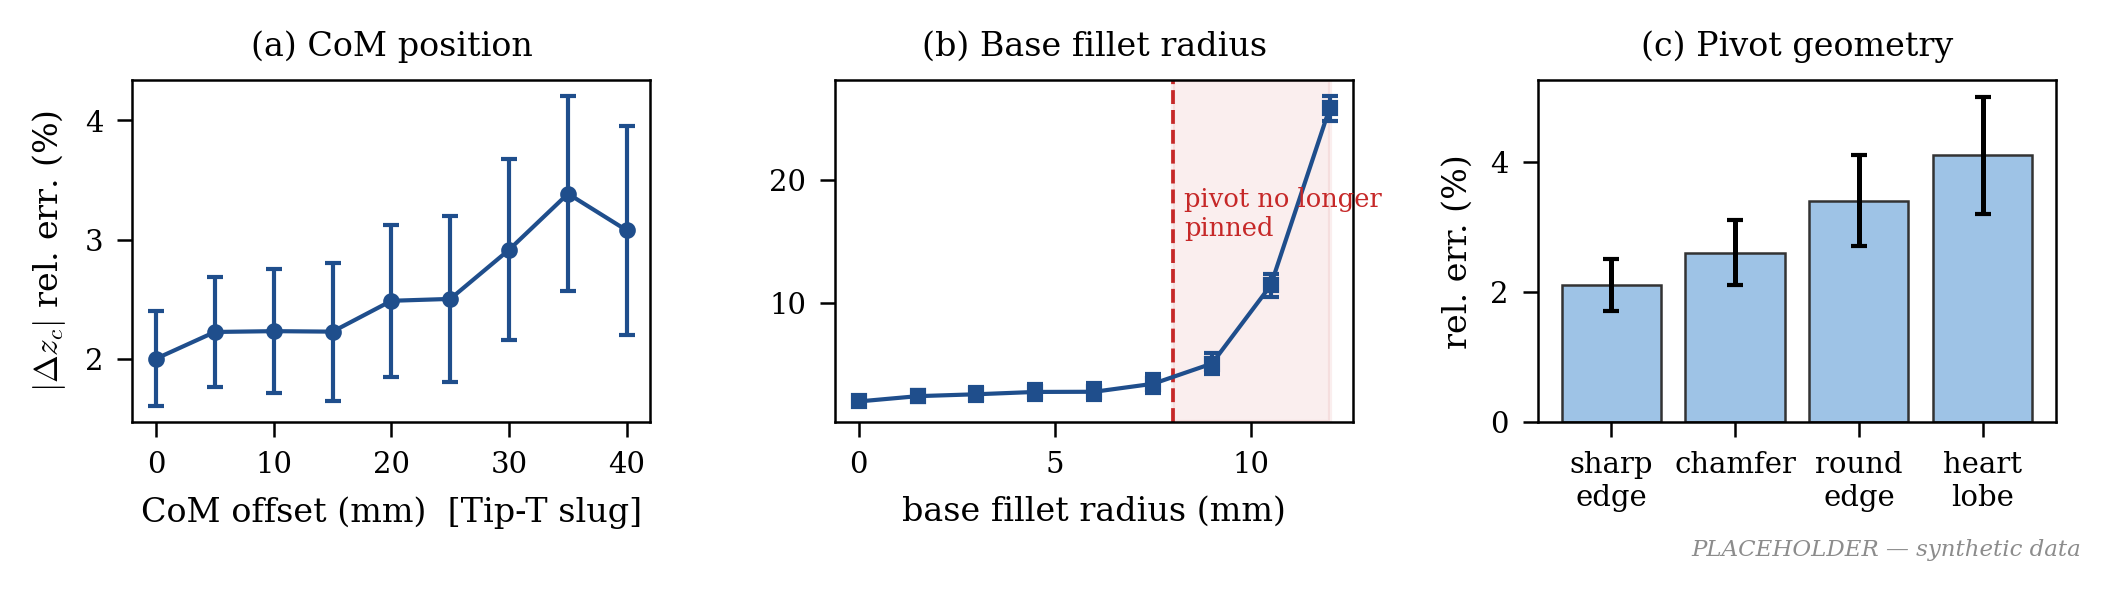
\includegraphics[width=0.95\linewidth]{figures/fig5_sweeps.png}
  \caption{Parametric sweeps. Estimation error versus (a) CoM offset, (b) base fillet radius, and (c) pivot geometry.}
  \label{fig:sweeps}
\end{figure}

\subsection{Safety framework validation}
We verify that executed interactions remain inside the admissible set \eqref{eq:admissible} and that the predictive margin prevents the slip hazard in cases where the reactive scheme of \cite{hyland_isrr} would retry or fail. Fig. \ref{fig:tradeoff} reports the safety--accuracy tradeoff: estimation error versus the certified $\eta_{\mathrm{safety}}$, and the realized per-arc trajectories of $\lambda_{\mathrm{topple}}$ (showing the sign flip at $\theta^{*}$) and $\lambda_{\mathrm{slip}}$ (the certified hazard), including cases where the arc is driven through $\theta^{*}$ under a favorable slip budget and cases where the slip limit binds first. We additionally report the logged finger-object friction-cone margin (Section \ref{sec:method}) across all trials, confirming the by-design assumption held throughout rather than merely assuming it.
\todo{Fill Fig. \ref{fig:tradeoff} with data --- this is the thesis-defining figure; prioritize at least one trace driven cleanly through $\theta^{*}$.}
\begin{figure}[t]
  \centering
  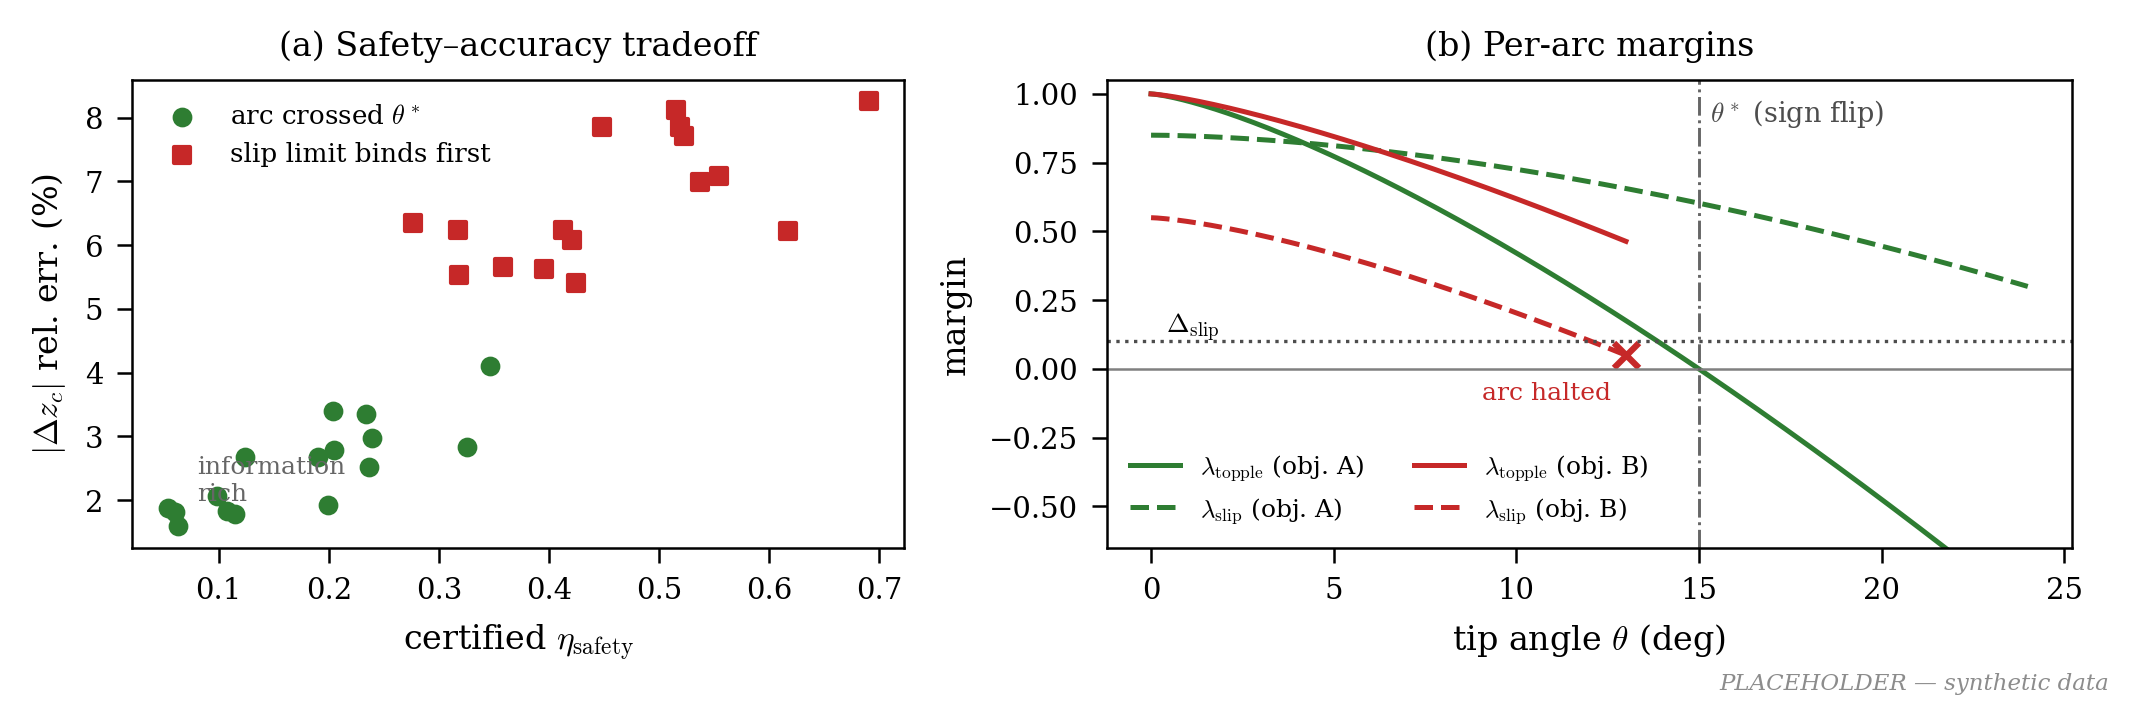
\includegraphics[width=0.95\linewidth]{figures/fig6_tradeoff.png}
  \caption{Safety--accuracy tradeoff. (left) Estimation error versus certified $\eta_{\mathrm{safety}}$. (right) Per-arc margins $\lambda_{\mathrm{topple}}(\theta)$ and $\lambda_{\mathrm{slip}}(\theta)$, illustrating both objects whose slip budget admits crossing $\theta^{*}$ ($\lambda_{\mathrm{topple}}$ changes sign while $\lambda_{\mathrm{slip}}$ stays positive) and objects where the slip limit binds first.}
  \label{fig:tradeoff}
\end{figure}

\subsection{Robustness}
Rather than an empirical noise-injection study, we report an analytic first-order sensitivity analysis: the Jacobian of $(m, z_c, \mu_t)$ with respect to the pose and geometry inputs used in the wrench balance, evaluated at the fitted operating point. We surface the press-moment-arm sensitivity of Section \ref{sec:conditioning} as a disclosed finding with a stated mitigation rather than a hidden weakness: because the press-induced moment about the pivot scales with $F_{\mathrm{press}}\cdot\delta r$, a small lever-arm localization error $\delta r$ under a large press can dominate the pull-torque signal that identifies $m$, which is precisely the rank-deficiency (force-correlated moment contamination) behavior we characterize, and argues for biasing the press toward the low end of $\mathcal{F}_{\mathrm{press}}$ during the estimation window rather than for abandoning the press. \todo{fill with the computed sensitivities/Jacobian values.}

\subsection{Complete-pipeline demonstration} 
For one to two objects we run planar $(x_c, y_c)$ estimation end-to-end (with accompanying video) so the full pipeline is exercised without a supplied planar CoM. This demonstrates completeness and is not a contribution of this work.

\subsection{Comparison}
Table \ref{tab:method_comparison} positions press-and-pull against method families qualitatively. We additionally implement a quantitative ablation against forward tipping on identical objects, and a multi-tip equi-effect baseline, isolating the contribution of the press and of the safety framework. The press's contribution is isolated by tipping success rate and recovered-parameter error on curved-edge, low-friction objects where forward tipping is infeasible by \eqref{eq:thresholds}; the safety framework's contribution is isolated by comparing the retry/failure rate of the reactive press loop of \cite{hyland_isrr} against the predictive certification of Section \ref{sec:method} on identical objects, together with estimation error reported at matched $\eta_{\mathrm{safety}}$ so accuracy differences are not confounded with differing safety margins. \todo{fill ablation numbers.}

\begin{table*}[htbp]
    \centering
    \caption{Comparison of qualitative method-families and capability matrix. ($\checkmark$ = yes, $\sim$ = partial/conditional, $\times$ = no, n/a = not applicable.)}
    \label{tab:method_comparison}
    \scriptsize
    \setlength{\tabcolsep}{2.2pt}
    \begin{tabular}{l l c c c c c c c l}
        \toprule
        \textbf{Method family} & \textbf{Sensing} & \textbf{Grasp-free} & \textbf{Shape-free} & \textbf{CoM ht.} & \textbf{Mass} & \textbf{Friction} & \textbf{Non-unif.\ density} & \textbf{Slip-cert.\ safety} & \textbf{Interactions} \\
        \midrule
        \textbf{Press-and-pull (ours)} & F/T + vision & \checkmark & \checkmark & \checkmark & \checkmark & \checkmark & \checkmark & \checkmark\textsuperscript{a} & single \\ \addlinespace
        Multi-tip / GEEP (Yu) & F/T + vision & \checkmark & $\times$ & \checkmark & \checkmark & $\times$ & $\sim$ & $\times$ & multiple \\ \addlinespace
        Forward tipping & F/T + vision & \checkmark & \checkmark & \checkmark & \checkmark & $\times$ & $\sim$ & $\sim$ (topple only) & single \\ \addlinespace
        Grasp-based excitation & F/T & $\times$ & $\sim$ & \checkmark & \checkmark & $\times$ & \checkmark & n/a & excitation \\ \addlinespace
        Planar pushing & F/T / vision & \checkmark & \checkmark & $\times$ & $\sim$ & $\sim$ & $\times$ & $\sim$ (avoids) & multiple \\ \addlinespace
        Tactile distribution & tactile & $\sim$ & \checkmark & \checkmark & $\sim$ & $\sim$ & \checkmark & depends & many \\ \addlinespace
        Vision-only / learned & vision & \checkmark & $\times$ & predicted & $\times$ & $\times$ & $\times$ & n/a & none \\ \addlinespace
        VLM + interaction (Phys2Real \cite{wang_phys2real_2026}) & vision + interaction & \checkmark & $\times$\textsuperscript{b} & $\sim$\textsuperscript{b} & $\sim$\textsuperscript{b} & $\sim$\textsuperscript{b} & \checkmark & n/a & multiple \\ \addlinespace
        \bottomrule
    \end{tabular}
    \\[3pt]
    {\footnotesize \textsuperscript{a}Press-and-pull additionally requires a reachable, visible top face for the press; where this is unavailable, forward tipping remains preferable. \textsuperscript{b}Relies on a VLM-inferred parameter prior refined by online interaction, rather than a model-free closed-form fit.}
    \todo{re-verify Phys2Real capability marks}
\end{table*}



%% ==============================================
%% Validation: parameter-gated manipulation
%% ==============================================
\section{Validation: Parameter-Gated Dynamic Shoving}
\label{sec:validation}
 
Accurate parameters are only useful if they change what the robot can safely do. We therefore close the loop with a downstream manipulation primitive whose success is \emph{gated} by the estimated parameters: a dynamic shove that drives an object into a target planar region. The goal region in $xy$ should be reached with an upright, no-tip orientation in a single push. Further, the goal region is beyond the reach of the robot arm such that the robot must break contact with the object while still in motion. This task is deliberately chosen since it cannot succeed without all three parameters, and so that the cost of \emph{not} knowing them is a visible, mechanically distinct failure rather than a quiet loss of accuracy.

\begin{figure}[t]
  \centering
  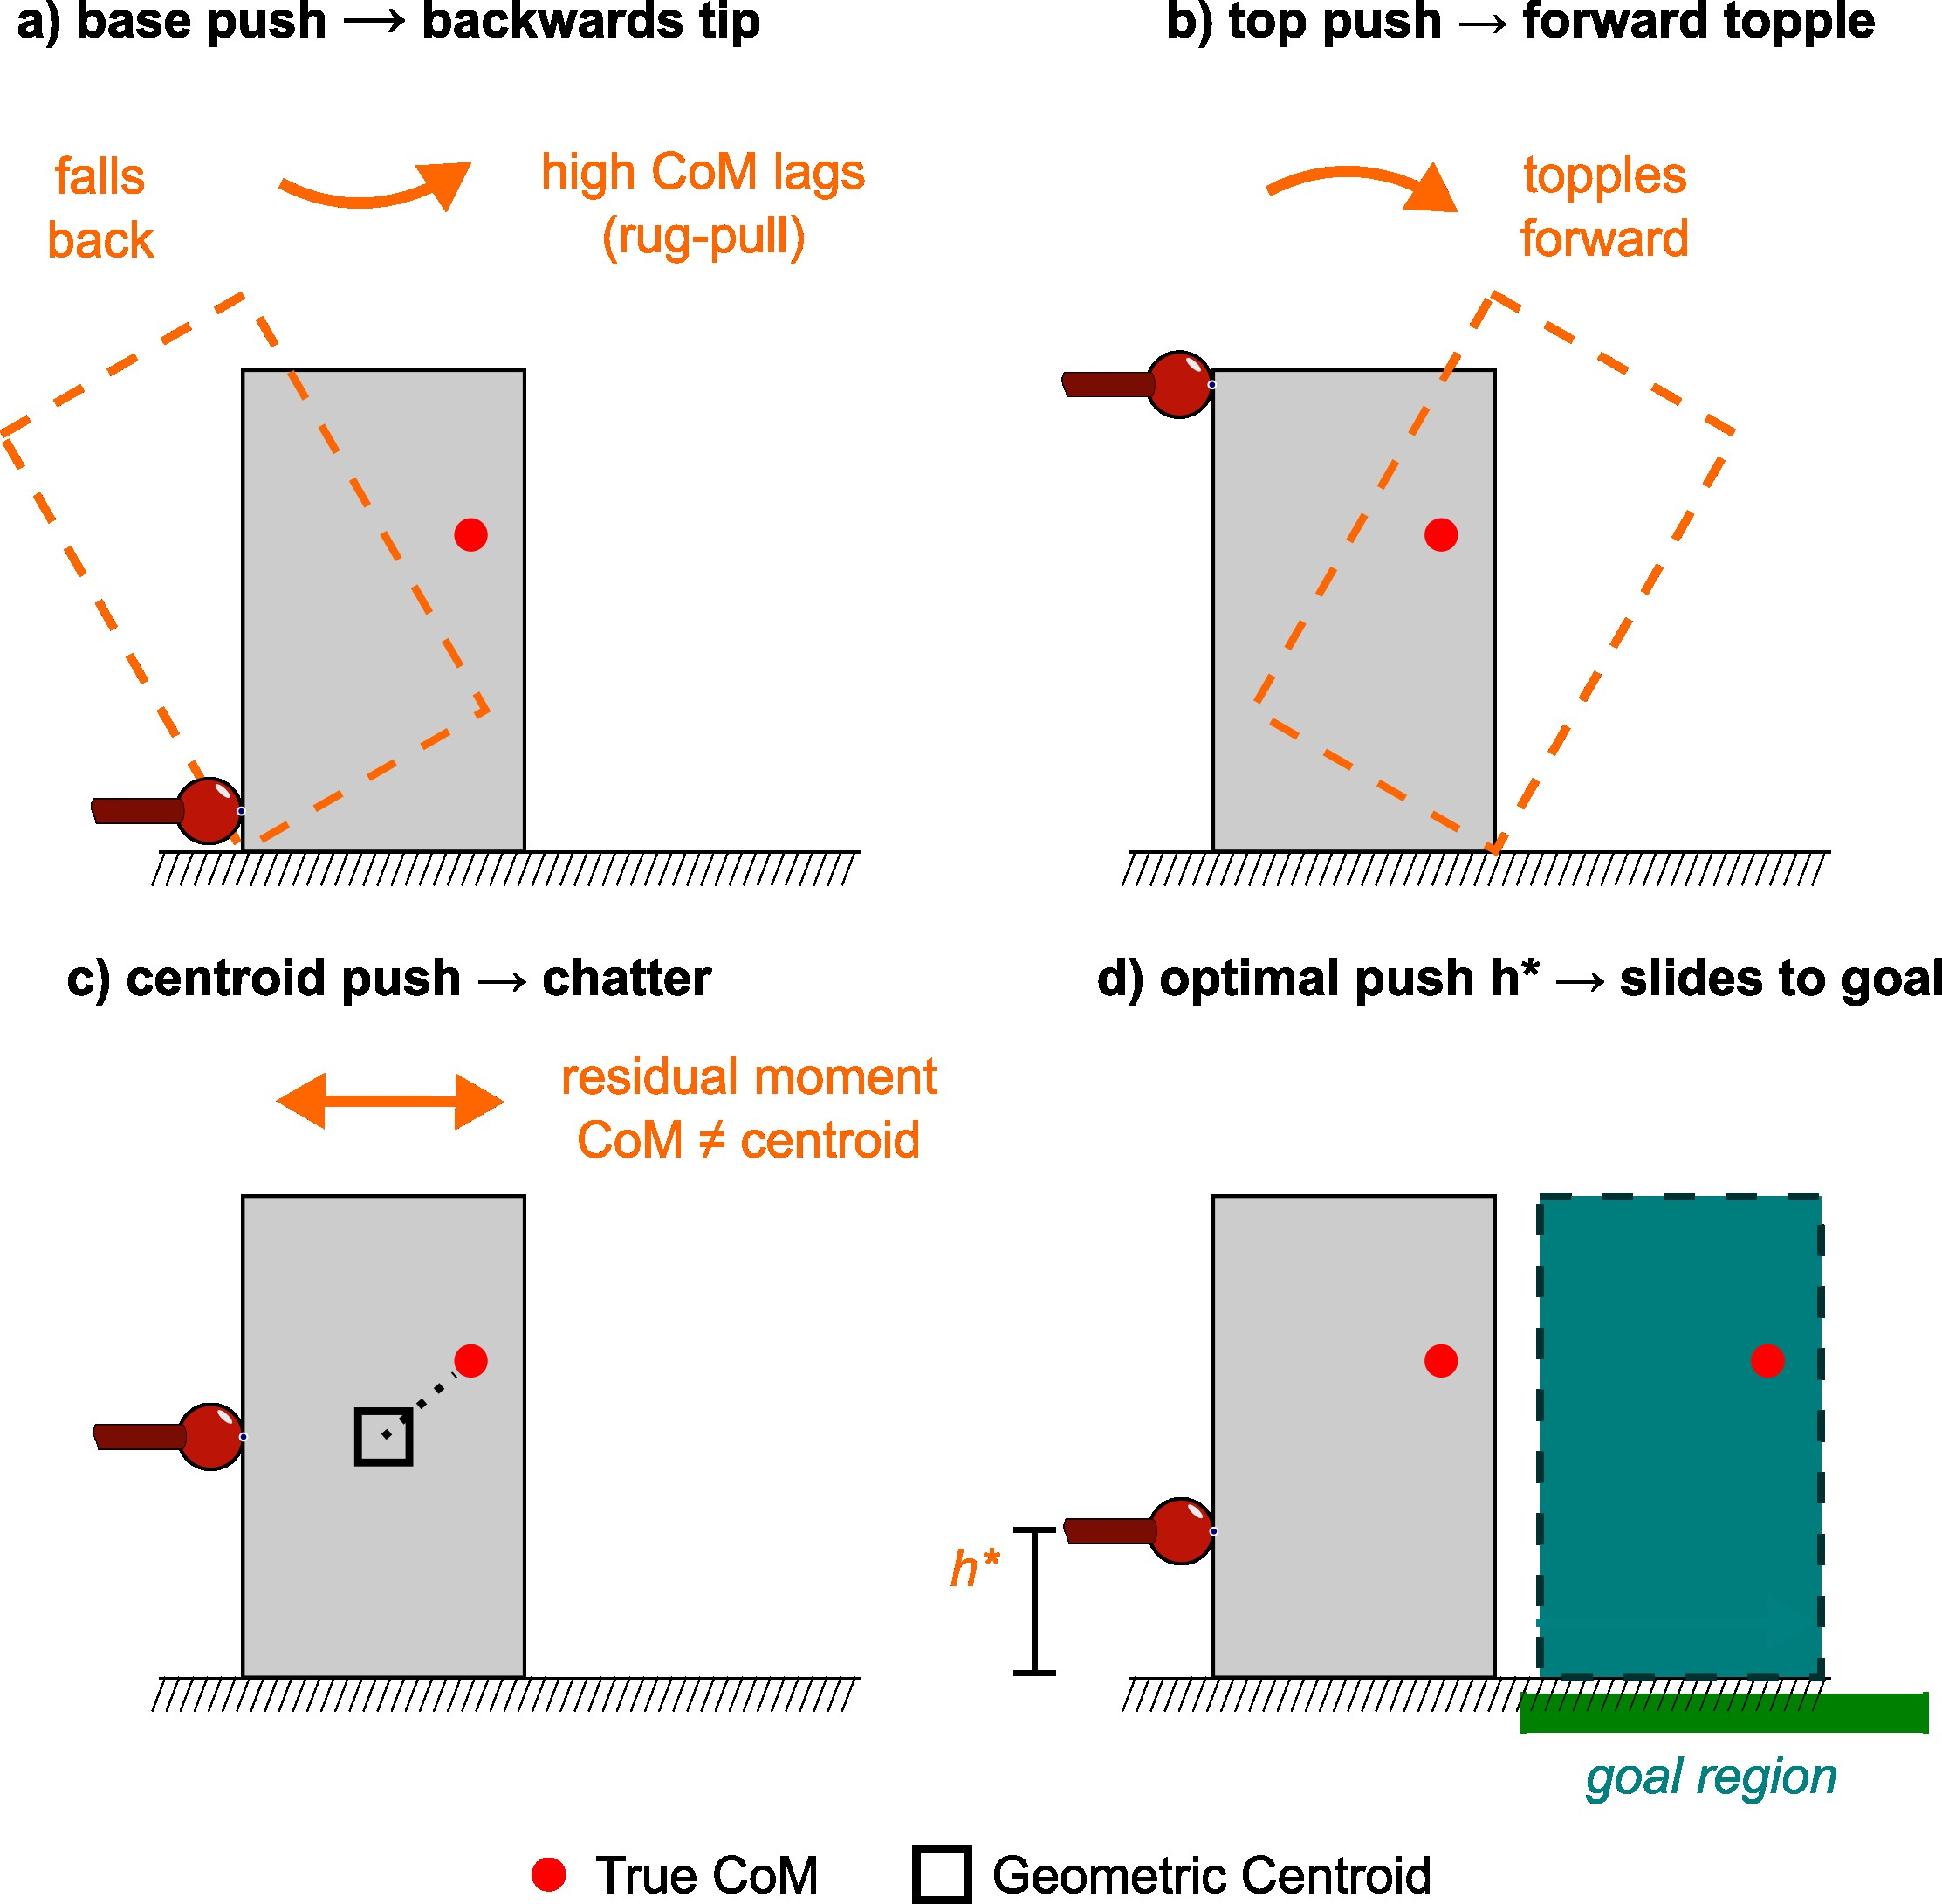
\includegraphics[width=0.98\linewidth]{figures/shove_validation.jpg}
  \\[4pt]
  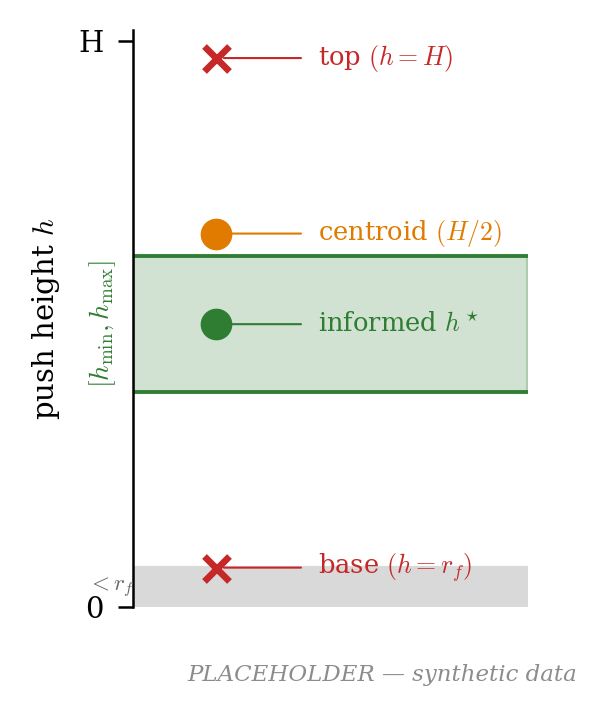
\includegraphics[width=0.6\linewidth]{figures/fig7_inset_window.png}
  \caption{Parameter-gated shove-to-region validation. Uninformed geometry-only push heuristics fail in distinct ways on a high-CoM, non-uniform object: (a) a base push tips it backward (rug-pull, the high CoM lags); (b) a top push topples it forward (push above the CoM, base friction pinning the bottom); (c) a centroid push chatters because the true CoM is offset from the geometric centroid. (d) The informed push, applied at the height $h^{*}$ computed from the estimated $(m, z_c, \mu_t)$ and within the no-tip window, slides the object cleanly into the target $xy$ region without tipping. (e) Inset: the admissible window $[h_{\min}, h_{\max}]$ with the four policies' push heights marked as points, so the gating claim is legible at a glance.}
  \label{fig:shove}
\end{figure}
 
\noindent \textbf{Why the task needs all three parameters}
Observing Figure \ref{fig:shove}, the shove is gated jointly by mass, CoM height, and friction, provided the task is executed in a control mode under which mass is genuinely load-bearing rather than merely limiting actuator effort (Section \ref{sec:shove_control}):
\begin{itemize}
  \item \textbf{CoM height $z_c$} locates the no-tip push-height window. A horizontal shove applied at height $h$ produces, together with the inertial reaction at the CoM and the friction reaction at the base, a net moment about the support edges; avoiding rotation constrains $h$ to an admissible window centered near $z_c$ under an aggressive shove. A high CoM therefore pushes the window up and leaves little margin, and the window cannot be located from geometry alone since the true $z_c$ and CoM offset are unknown a priori.
  \item \textbf{Mass $m$} sets the force needed to reach the target region against base friction, and scales the inertial moment that the no-tip constraint must absorb.
  \item \textbf{Friction $\mu_t$} sets the deceleration after release, and hence the stopping distance into the target region, and governs the competition between sliding and tipping at contact.
\end{itemize}

\paragraph{No-tip condition and admissible push height}
We make the analysis concrete in the vertical plane containing the push. Let the support base reduce to the segment $[-d_r, d_f]$, where $d_r$ and $d_f$ are the horizontal distances from the CoM's vertical projection to the trailing and leading bottom edges; non-uniform density appears precisely as an asymmetry $d_f \neq d_r$. The object slides under a purely horizontal shove of constant acceleration $a$ applied at height $h$, with a single Coulomb coefficient $\mu_t$ (taken equal in stick and slip, consistent with the estimator). Vertical balance gives $N = mg$, and horizontal balance $F - \mu_t N = ma$ gives the required push force
\begin{equation}
    F = m\,(a + \mu_t g).
    \label{eq:shove_force}
\end{equation}
For pure translation the angular acceleration is zero, so the moments about the CoM must vanish. Balancing the push moment $(z_c - h)F$, the friction-drag moment $-z_c \mu_t N$, and the ground-reaction moment $x_{cp} N$ locates the center of pressure:
\begin{equation}
    x_{cp}(h) = \mu_t h - \frac{(z_c - h)\,a}{g}
              = \Big(\mu_t + \tfrac{a}{g}\Big)\,h - \frac{z_c\, a}{g},
    \label{eq:cop}
\end{equation}
which is linear and strictly increasing in $h$: pushing higher drives the center of pressure forward, pushing lower drives it back. The object slides without tipping iff the center of pressure stays within the support base, $-d_r \le x_{cp}(h) \le d_f$, which solves to the admissible push-height window
\begin{equation}
    h_{\min} = \frac{a\,z_c - g\,d_r}{a + \mu_t g}, \qquad
    h_{\max} = \frac{a\,z_c + g\,d_f}{a + \mu_t g},
    \label{eq:hwindow}
\end{equation}
intersected with the physically reachable range $[r_f, H]$, where $H$ is the object height and $r_f$ is the finger radius, which excludes the unreachable bottom sliver rather than the geometrically convenient but unreachable $h=0$. The window has width $g\,(d_f + d_r)/(a + \mu_t g)$, and the maximum-margin push height is its midpoint,
\begin{equation}
    h^{\star} = \frac{a\,z_c + \tfrac{1}{2}\,g\,(d_f - d_r)}{a + \mu_t g}
    \;\xrightarrow[\;d_f=d_r\;]{}\; \frac{a\,z_c}{a + \mu_t g},
    \label{eq:hstar}
\end{equation}
which centers the center of pressure in the base. Equations \eqref{eq:cop}--\eqref{eq:hstar} make the parameter dependence explicit: the window is located by $z_c$, scaled by $\mu_t$ and the base geometry, and traversed by the acceleration $a$ that $m$ and \eqref{eq:shove_force} convert into a force. This is the same slide-versus-tip competition of \eqref{eq:thresholds}, now imposed as a constraint to satisfy rather than a mode to select. Equations \eqref{eq:cop}--\eqref{eq:hstar} are written for a commanded acceleration $a$; they hold for either control mode discussed next, and are the natural form under stiff position/velocity control, where $a$ is the directly commanded quantity.

Two limits confirm the mechanics. As $a \to \infty$ the window collapses, $h_{\min}, h_{\max} \to z_c$: an aggressive shove can avoid tipping only by pushing through the CoM height, so a high, poorly known $z_c$ is the binding difficulty. As $a \to 0$ the upper bound recovers the classical quasistatic block-tipping threshold $h_{\max} \to d_f/\mu_t$, while $h_{\min} \to -d_r/\mu_t < 0$ falls below the table --- backward tipping is therefore an intrinsically dynamic, rug-pull effect with no quasistatic analogue. \todo{$d_f, d_r$ come from the convex-hull footprint and the estimated CoM projection; confirm the purely-horizontal-push and constant-$a$ assumptions hold on the rig, and add a vertical-push-component term if the finger imparts one.}

\paragraph{Execution mode, shove intensity, and why mass is load-bearing} \label{sec:shove_control}
Equations \eqref{eq:hwindow}--\eqref{eq:hstar}, and the post-release coast distance $v^2/(2\mu_t g)$ derived below, contain $a$, $z_c$, $\mu_t$, and the base geometry, but \emph{no $m$}: under stiff position/velocity control --- the natural mode on our arm --- the commanded trajectory fixes $a$ directly, mass cancels out of the moment balance, and mass would gate the task only through the actuator's force limit via \eqref{eq:shove_force}, a weak and easily attacked version of the claim that the task needs all three parameters. We therefore execute the shove force-controlled (a commanded force profile $F$, or admittance with a force target), so that $a = F/m - \mu_t g$ and every governing quantity is jointly parameterized by $(m,\mu_t,z_c)$. Define the dimensionless \emph{shove intensity}
\begin{equation}
    \boxed{\ \sigma \;\equiv\; \frac{F}{\mu_t m g} \;=\; 1 + \frac{a}{\mu_t g} \;\ge\; 1\ }, \label{eq:sigma}
\end{equation}
with $\sigma=1$ incipient sliding ($a=0$) and large $\sigma$ an aggressive shove. Substituting $a = \mu_t g(\sigma-1)$ into \eqref{eq:hwindow}--\eqref{eq:hstar} rewrites the window purely in terms of $\sigma$,
\begin{equation}
    h_{\min,\max} = z_c\Big(1-\tfrac{1}{\sigma}\Big) \mp \frac{d_{r,f}}{\mu_t\,\sigma}, \qquad
    w = \frac{d_f+d_r}{\mu_t\,\sigma}, \label{eq:sigma_window}
\end{equation}
and, for a shove from rest with constant force over stroke $d_{\mathrm{push}}$, the release velocity $v^2 = 2ad_{\mathrm{push}}$ gives a coast distance $v^2/(2\mu_t g) = (\sigma-1)d_{\mathrm{push}}$, so the total travel to the target is
\begin{equation}
    \boxed{\ D \;=\; \sigma\, d_{\mathrm{push}}\ }. \label{eq:overreach}
\end{equation}
The same scalar $\sigma$ is simultaneously the normalized push force, the normalized acceleration, and the \emph{overreach ratio} $D/d_{\mathrm{push}}$: it collapses what looks like a three-parameter planning problem into one knob, wider windows and gentler shoves at small $\sigma$ trading against shorter, more aggressive strokes at large $\sigma$ --- the shove-side structural analog of the safe press band of Section \ref{sec:method}. With $F = \sigma \mu_t m g$ and \eqref{eq:overreach}, $D = F d_{\mathrm{push}}/(\mu_t m g)$, so to first order the placement error decomposes cleanly as
\begin{equation}
    \frac{\Delta D}{D} \;\approx\; -\frac{\Delta\mu_t}{\mu_t} - \frac{\Delta m}{m}, \label{eq:placement_error}
\end{equation}
giving a crisp division of labor: $(\mu_t,m)$ gate placement, $(z_c,\mu_t,m)$ gate tipping, and every estimated parameter is load-bearing under this execution mode.

\paragraph{Coast-phase feasibility gate}
Section \ref{sec:method}'s certification covers only the analog of the push phase; the coast phase after release has its own, push-independent, no-tip condition. Setting $F=0$ in the moment balance underlying \eqref{eq:cop} removes the push term entirely, leaving the ground-reaction and friction-drag moments to balance on their own: $x_{cp}^{\mathrm{coast}} = \mu_t z_c$, independent of $h$, $a$, and $F$. The object coasts to rest without tipping forward iff
\begin{equation}
    \boxed{\ \mu_t\, z_c \;\le\; d_f\ }, \label{eq:coast_gate}
\end{equation}
the classical decelerating-block criterion. No choice of push height or intensity can rescue an object that violates \eqref{eq:coast_gate}: it gates object/face feasibility, not push planning, and must be checked as a precondition before planning $h$ and $\sigma$. It is $d_f$, the \emph{leading} CoM-to-edge distance, that binds, so the dangerous configuration is a CoM shifted toward the push direction --- precisely the non-uniform-density case in Fig.~\ref{fig:shove}. This formalizes face selection as the discrete choice $\max_{\text{face}}\big(d_f(\text{face}) - \mu_t z_c\big)$ using the estimated planar CoM to compute $d_f$ per face from the footprint hull. If both the push-phase CoP \eqref{eq:cop} and the coast-phase CoP \eqref{eq:coast_gate} lie inside the base, release involves no impulsive rotation for a rigid body; in practice this also requires the finger to brake at $|a_{\mathrm{brake}}| > \mu_t g$ so the object actually leaves contact rather than being decelerated by the finger itself.

\paragraph{Unified shove margin}
Mirroring the estimation-side margin of Section \ref{sec:method}, define a normalized no-tip margin
\begin{equation}
    \lambda_{\mathrm{tip}}(x_{cp}) = \frac{\min\big(d_f - x_{cp},\ x_{cp}+d_r\big)}{(d_f+d_r)/2} \in (-\infty,1], \label{eq:lambda_tip}
\end{equation}
equal to $1$ when the CoP is centered and $0$ at incipient tip about either edge. Evaluating it in both phases and taking the worst case gives a single certificate for the whole shove,
\begin{equation}
    \eta_{\mathrm{shove}} = \min\big\{\, \lambda_{\mathrm{tip}}(x_{cp}(h)),\ \lambda_{\mathrm{tip}}(\mu_t z_c) \,\big\}, \label{eq:eta_shove}
\end{equation}
admissible iff $\eta_{\mathrm{shove}} \ge \Delta_{\mathrm{tip}}$. The estimation interaction is certified by the single slip margin $\eta_{\mathrm{safety}}$ of \eqref{eq:eta}; the downstream task it enables is certified by the single tip margin $\eta_{\mathrm{shove}}$, and both trade conservatism against performance through one scalar, $\Delta_{\mathrm{slip}}$ on the estimation side and $\sigma$ on the task side --- the demonstration is part of the same framework, not an appendix to it.

\paragraph{Uninformed baselines and their failure modes}
Without the estimated parameters, a system defaults to geometry-only push heuristics, each of which fails on a high-CoM, non-uniform object in a distinct way (Fig.~\ref{fig:shove}), and each failure is a prediction from \eqref{eq:hwindow} rather than only an observation: a base push ($h=r_f$) is predicted to tip the object \emph{backward} about its trailing edge whenever $r_f < h_{\min}$ (the rug-pull effect: the base is driven forward while the high CoM lags); a top push ($h=H$) is predicted to topple the object \emph{forward} about its leading edge whenever $H > h_{\max}$ (base friction pins the bottom); and a centroid push ($h=H/2$, assuming the incorrect symmetric $d_f=d_r$) is predicted to sit outside the true asymmetric window, and \emph{chatter} between incipient slip and incipient tip, whenever $|H/2-h^{\star}|>w/2$. Only the informed push, applied within the estimated no-tip window, slides the object cleanly into the target region.

\paragraph{Note on the static-to-dynamic transfer}
The parameters are estimated quasistatically, but the shove is dynamic. The demonstration thus also tests whether quasistatically recovered $(m, z_c, \mu_t)$ transfer to a dynamic regime --- including the implicit assumption of a single friction coefficient across static and kinetic contact. We report this transfer rather than assume it.

\paragraph{Planar (yaw) alignment}
The analysis above assumes the push line passes through the CoM's vertical plane. A lateral offset $e_y$ between the push line and the estimated planar CoM $(x_c,y_c)$ produces a yaw moment resisted by the base-friction distribution rather than the vertical-plane no-tip constraint above; rather than model it, we impose the alignment condition $e_y \le \bar e_y$, use the estimated planar CoM (from the slide mode) to align the informed policy, and report final yaw error as a metric. Uninformed centroid alignment inherits the same CoM-vs.-centroid error in yaw, strengthening the chatter/yaw failure story of the centroid baseline above.

\paragraph{Uncertainty gating: from estimator error to guaranteed success}
The estimator's Table \ref{tab:results} errors propagate to the shove in closed form through two channels. Writing the push-phase CoP in force-controlled form, $x_{cp}(h) = \mu_t z_c - (z_c-h)F/(mg)$ (algebraically \eqref{eq:cop} with $a=F/m-\mu_t g$ substituted), its first-order sensitivities at fixed $F,h$ are
\begin{equation}
    \frac{\partial x_{cp}}{\partial z_c} = -\mu_t(\sigma-1), \quad
    \frac{\partial x_{cp}}{\partial \mu_t} = z_c, \quad
    \frac{\partial x_{cp}}{\partial m} = \frac{F(z_c-h)}{m^2 g}. \label{eq:tip_sensitivity}
\end{equation}
No-tip is guaranteed despite estimation error if the worst-case CoP shift stays inside the planned half-window slack,
\begin{align}
    &\mu_t(\sigma-1)\,\varepsilon_{z_c} + z_c\,\varepsilon_{\mu_t} + \frac{F|z_c-h^{\star}|}{m^2 g}\,\varepsilon_m \notag \\
    &\hspace{4em}\le\; \tfrac{1}{2}w - |\text{planned offset}|, \label{eq:tip_gate}
\end{align}
where $\varepsilon_{(\cdot)}$ are the (absolute) Table \ref{tab:results} error bounds. Note $\partial x_{cp}/\partial z_c \propto (\sigma-1)$: a gentler shove is not only wider-windowed by \eqref{eq:sigma_window} but also less sensitive to $z_c$ error, closing the loop on the press-schedule-style policy of Section \ref{sec:method}: \eqref{eq:tip_gate} states exactly how much to lower $\sigma$ given the certified estimate error. The placement channel follows from \eqref{eq:placement_error}: guarantee region-reach with a goal half-width
\begin{equation}
    \delta \;\ge\; D\,(\varepsilon_{\mu_t} + \varepsilon_m)\cdot k, \qquad k \gtrsim 1. \label{eq:delta_gate}
\end{equation}

\paragraph{Protocol and metrics}
We use a high-CoM, non-uniform-density object (e.g.\ the Tip-T) so the failure modes are well separated. Rather than choosing the goal region and $\sigma$ arbitrarily, we choose them from \eqref{eq:tip_gate} and \eqref{eq:delta_gate} using the \emph{measured} Table \ref{tab:results} errors: the goal half-width $\delta$ is set by \eqref{eq:delta_gate}, and $\sigma$ (equivalently, the slug offset used to build the test object) is chosen so the three uninformed heuristics of the preceding paragraph violate the window by more than the measurement error, making their predicted failure a consequence of the certificate rather than an incidental observation. For each policy --- base, top, centroid, and informed --- we report the a-priori prediction (tip / no-tip, region-reach / miss) from \eqref{eq:hwindow}--\eqref{eq:eta_shove} alongside the observed outcome, final yaw error, and success rate over $N\ge10$ trials per policy; that prediction-vs.-outcome table is the parameter-gated-feasibility claim. The entire planning problem above --- selecting a face via \eqref{eq:coast_gate}, a height via \eqref{eq:sigma_window}, and an intensity via the stroke limit $\sigma \ge D/L$ for reach $L$ --- is closed-form, with no learned or search-based component, consistent with the framework's broader thesis of more affordance from less information; we leave a full closed-loop planner over $(\text{face},\sigma,h)$ to future work.


%% ==============================================
%% Conclusion
%% ============================================== 
\section{Conclusions} \label{sec:conclusion}

We presented a criticality-aware safety framework for non-prehensile parameter estimation that identifies press-induced object--table slippage as the single governing hazard, shows that toppling is a consequence of that same slip constraint rather than an independent risk, and certifies an interaction against it. Built on the press-and-pull primitive, the framework recovers mass, CoM height, and friction in closed form from limited, geometry-free interactions, while keeping the motion inside an admissible set defined by a single, predictive safety margin --- one that, when an object's slip budget allows, permits deliberately crossing the nominal toppling angle to sharpen the recovered CoM height rather than only approaching it asymptotically. The central structural insight is that the press force which guarantees tipping early in the arc injects a horizontal load that grows with the tip angle, so safety is a constrained trajectory problem with a bounded safe press band rather than a monotone "more press is safer" rule. We showed the same estimates are actionable by gating a downstream dynamic shove-to-region task with an analogous closed-form certificate: a single dimensionless shove intensity $\sigma$ governs the speed--safety tradeoff, a push-independent coast-phase gate is a precondition on face selection, and the estimator's error bounds convert directly into guaranteed task tolerances --- the two certificates, $\eta_{\mathrm{safety}}$ at estimation time and $\eta_{\mathrm{shove}}$ at task time, are the same principle applied on either side of the interaction.

The applicability envelope is explicit. The press requires a reachable, visible top face; where that is unavailable, forward tipping remains preferable. Base curvature is tolerated up to the range characterized by the fillet sweep, beyond which the pivot can no longer be pinned. The shove additionally requires the coast-phase gate $\mu_t z_c \le d_f$ to hold on at least one face. Within these bounds the framework recovers all three parameters with relative errors under \todo{X\%} while remaining certifiably safe.

\paragraph{Future work} Three extensions follow naturally: relaxing the rigid-body assumption toward quasistatic fluid redistribution in partially filled containers, which would additionally enable fluid-height estimation; extending beyond the fillet range to arbitrary convex or rocking bottoms, likely via a dual-contact ("fork") end-effector, which would also let an explicit, instrumented finger--face slip margin replace the current design-time assumption of a sufficiently pressed, high-friction fingertip; and folding the covariance coupling into a closed-loop controller that selects the press within $\mathcal{F}_{\mathrm{press}}$ online and the shove intensity $\sigma$ online, together with the empirical validation of that coupling. \todo{advisor decision: fluid as future work vs. results section.}

\ifCLASSOPTIONcaptionsoff
  \newpage
\fi

\bibliography{references.bib}

\end{document}